
\chapter{基于粒子群算法的软件补偿方法及算法硬化}
\section{粒子群算法}
\label{粒子群算法}
\subsection{粒子群算法基本原理}

粒子群算法(Particle Swarm optimization,PSO)是一种启发于鸟群协同捕食行为的智能算法,利用种群与个体之间的信息交互来寻找问题的最优解,具有较高的搜索效率和精度\cite{潘红丽2022基于改进粒子群算法的垃圾清运车辆低碳路径规划},已广泛应用于函数优化等领域\cite{2022Environmental}。
\begin{figure}[htb]
  \centering
  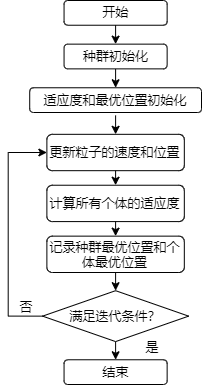
\includegraphics[width=4cm,height=7cm]{fig/4-fig/粒子群算法流程图.png}
  \caption{粒子群算法流程图}
  \label{fig:粒子群算法流程图}
\end{figure}

可以假设这样一个场景:一群鸟在随机的搜寻食物,并且搜寻空间里只有一块食物,所有的鸟都不知道食物在哪里,并且所有鸟的初始位置和搜寻方向都是随机的。在该场景下,一个找寻食物的最优策略就是搜寻离食物最近的鸟的周围。距离食物的距离就代表着优化效果的好坏,而鸟群每个时刻所处在的位置,就代表着粒子群算法覆盖到的迭代值,整个空间即为粒子群算法的搜索空间,将该方式抽象成算法,如图\ref{fig:粒子群算法流程图}所示。

由图\ref{fig:粒子群算法流程图}中可以看出,粒子群算法的第一步是对种群进行初始化,即设定优化对象的迭代起点,并根据目标函数计算出与起点对应的适应度(Fitness,下文简称fit),并在所有个体的适应度中筛选出最优的,用其对应的迭代起点作为整个种群目前的种群最优解(Global best,下文简称gbest),而所有个体的个体最优解(Person best,下文简称pbest),这样就完成了整个算法的初始化。随后使用gbest、pbest对粒子的速度和位置更新进行控制,使迭代方向不断朝着最优的方向进行,即上述“搜寻离食物最近的鸟的周围”的策略,具体的速度更新公式和位置更新公式如下式所示:
\begin{equation}\label{eq:粒子群算法速度更新}
  V^{k+1}_i=\omega V^{k}_i\,+\,c_pr_{and}(pbest_i-X^{(k)}_i)+c_gr_{and}(gbest\,-\,X^{(k)}_i).
\end{equation}
\begin{equation}\label{eq:粒子群算法位置新}
    X^{k+1}_i\,=\,X^{(k)}_i\,+\,V_i^{k+1}.
\end{equation}

上式中\(V^{k}_i\)和\( X^{k}_i\)中分别表示粒子的速度和位置,下标i表示种群中第i个粒子,上标(k+1)表示当前种群为第(k+1)次迭代,\(\omega\)称为惯性因子,是一个衡量全局寻优能力和局部寻优能力的非负参数;\(c_p\)和\(c_g\)为非负常数,通常设为2;、\(r_{and}\)为[0,1]范围内的随机数,\(pbest_i\)为第个粒子的个体历史最优位置,gbest为整个种群的历史最优位置。

\subsection{线性惯性权值递减策略}
由式\eqref{eq:粒子群算法速度更新}可以看出惯性因子主要控制粒子的历史速度对当前速度的影响,历史速度在当前速度中占比大,则速度的更新将主要集中在历史速度附近,此时粒子群算法的局部寻优能力较强,并且收敛速度较快;若历史速度在当前速度中占比小,则速度的更新将在整个搜索域中进行,此时粒子群算法的全局寻优能力较强,使得搜索结果容易跳出局部优值。

为了在迭代初期,能够有更好的全局寻优能力,尽可能找到搜索域中所有可能的最优解,在迭代后期拥有更好的局部寻优能力,以便快速收敛,在惯性因子的取值上采用线性递减策略\cite{冯浩2015一种改进的粒子群优化算法惯性权值递减策略},即惯性因子\(\omega\)由下式更新。
\begin{equation}\label{eq:omega更新公式}
  \omega^k\,=\,\omega_e\,+\,\frac{(\omega_i\,-\,\omega_e)(k_{max}\,-\,k)}{k_{max}}.
  \end{equation}

其中\(\omega_i\)和\(\omega_e\)分别为迭代开始时的惯性因子和迭代结束时的惯性因子,\(k_{max}\)为最大迭代次数,k为当前的迭代次数。通过对惯性因子使用线性递减策略,可以在迭代过程中不断调整全局寻优能力和局部寻优能力。

但是粒子群算法存在早熟收敛的问题,即当粒子群到达局部最优解附近时,粒子速度的更新主要由自身速度决定,并且由于粒子群算法的惯性因子\(\omega^k\)通常小于1,使得粒子速度的更新幅度将会越来越小,难以跳出该局部最优解\cite{范培蕾2009克服早熟收敛现象的粒子群优化算法}。

虽然Edlen公式的诞生方法使其补偿精度和使用条件受到一定影响,但原始的Edlen公式为PSO算法提供了一个优秀的搜索起点,相当于大幅压缩了PSO算法的搜索空间,这能非常有效地避免早熟收敛问题的出现。

\section{基于粒子群算法优化后的Edlen公式补偿方法}
为了解决上述的Edlen公式存在的问题,本文提出一种使用粒子群算法对Edlen公式进行优化的方法。

对于粒子群算法而言,目标函数的形式会严重影响算法优化的结果,而Edlen公式作为一个几十年来广泛使用的经验公式,虽然由于其诞生条件的局限性使得其使用范围受限,但Edlen公式的形式仍然具有重要的借鉴意义,将Edlen公式与粒子群算法相结合,不仅可以有效地避免粒子群算法寻找到局部最优解,避免早熟收敛现象的发生,还可以减小搜索空间,减小收敛时间,保证训练时不会影响实时数据测量及补偿。
\subsection{数据预处理}
使用粒子群算法对Edlen公式进行优化的第一步是对位移、温度、气压数据进行预处理,这点主要是基于下面两点考虑:
\begin{enumerate}
  \item 虽然所有被测量的采样周期均为$2s$,但是由于位移测量的上位机采用C-SHOP编写,而温度测量的上位机是基于LabVIEW开发的,气压测量主要依靠PACE1000气压传感器,这导致三者在定时功能上可能会有细微差别,而导致最终采样的点数不相同,所需要进行数据的裁剪。
  \item 出于不漏采任何有效信息,所以将采样周期设置为$2s$,但是温度和气压都是缓变量,并不可能在这么短的时间内明显变化,所以为了数据的可靠性,避免偶然性数据造成训练效果降低,需要对数据进行均值滤波。
\end{enumerate}
在进行数裁剪的时候采用如下策略:将位移、温度、气压三组中数据个数最少的作为基准,计算另外两组数据个数与基准的差值,这个差值即为需要裁剪的数据个数,将数据个数除以裁剪个数,然后向下取整即可得到每组数据对应的裁剪窗口长度,在每个裁剪窗口内将最后两个数取平均值,用平均值代替这两个数,这样即可实现数据裁剪。

在进行均值滤波的时候采用如下策略:取窗口长度为$30s$,即15个数据点,在整个数据段内进行滑动窗口的均值滤波。

\subsection{使用粒子群算法进行数据训练}
将式\eqref{eq:线性形式的Edlen公式}作为粒子群算法的目标函数,温度因子$\frac{\delta n}{\delta T}$和气压因子$\frac{\delta n}{\delta P}$作为两个搜索目标,第一次迭代的搜索起点分别为$-9.36*10^{-7}$和$2.68*10^{-9}$,即搜索点由下式更新:
\begin{equation}\label{eq:搜索点更新公式}
  \delta^{(n+1)}_i = \delta^{(n)}_i+(\delta^{(n)}_o-\delta^{(n)}_i).
  \end{equation}

式\eqref{eq:搜索点更新公式}中$\delta^{(n+1)}_i$为第$n+1$次训练时温度因子、气压因子初始搜索点,即$\delta_i\,=\,(\frac{\delta n}{\delta T}\,\,\,\frac{\delta n}{\delta P})$,所以该式描述的是第$n+1$的搜索起点与第$n$次搜索起点之间的关系。特别地,当$n=0$时,即第一次搜索的搜索起点为$\delta_i\,=\,(-9.36*10^{-7}\,\,\,2.68*10^{-9})$,即原始Edlen公式的温度因子值和气压因子值。$\delta_o^{(n)}$为第$n$次训练后粒子群算法计算出的温度因子和气压因子。

而每次训练计算$\delta_o^{(n)}$的适应度时,采用均方根误差作为评价指标,其计算方法如式\eqref{eq:均方根误差计算公式}所示:
\begin{equation}\label{eq:均方根误差计算公式}
  RMSE = \sqrt{\frac{\sum_{i=1}^{N}(x-\widehat x)^2}{N}}.
  \end{equation}


\section{整段式粒子群算法补偿效果}
将一整组的测量数据作为粒子群算法的训练样本,从给定的搜索起点开始,根据式\eqref{eq:均方根误差计算公式}计算初始适应度,并且进行种群最优位置和个体最优位置的初始化,然后根据式\eqref{eq:粒子群算法速度更新}和式\eqref{eq:粒子群算法位置新}更新种群中所有个体的速度和位置,然后循环迭代多次,直至达到迭代次数上限,此时种群的最优位置即为粒子群算法优化后的Edlen公式中的温度因子和气压因子,然后对测量数据进行补偿。训练样本统一使用测量臂长度$90nm$的干涉仪的测量数据,使用优化结果对测量臂长度$45nm$和$90nm$测量数据同时进行补偿,补偿结果如下。

\subsection{短时测量}
如图\ref{fig:粒子群算法优化后的短时测量补偿效果}所示,(a)图为测量臂长度为$45nm$的位移测量数据,(b)图为测量臂长度为$90nm$的位移测量数据,(c)图为对应的温度和气压数据,(a)、(b)、(c)三图的横轴均为时间,单位为h;(a)和(b)图中的竖轴为位移数据,单位为$nm$,其中带圆圈标注的蓝色曲线为原始的位移测量数据,带黄色方块标注的为使用原始Edlen公式补偿后的位移数据,带红色菱形标注的为使用粒子群算法优化后的补偿后位移数据,(c)图的竖轴为温度和气压数据,单位为$^{\circ}C$和$kPa$,其中带圆圈标注的蓝色曲线为温度数据,红色曲线为气压数据。
\begin{figure}[htb]
    \centering
    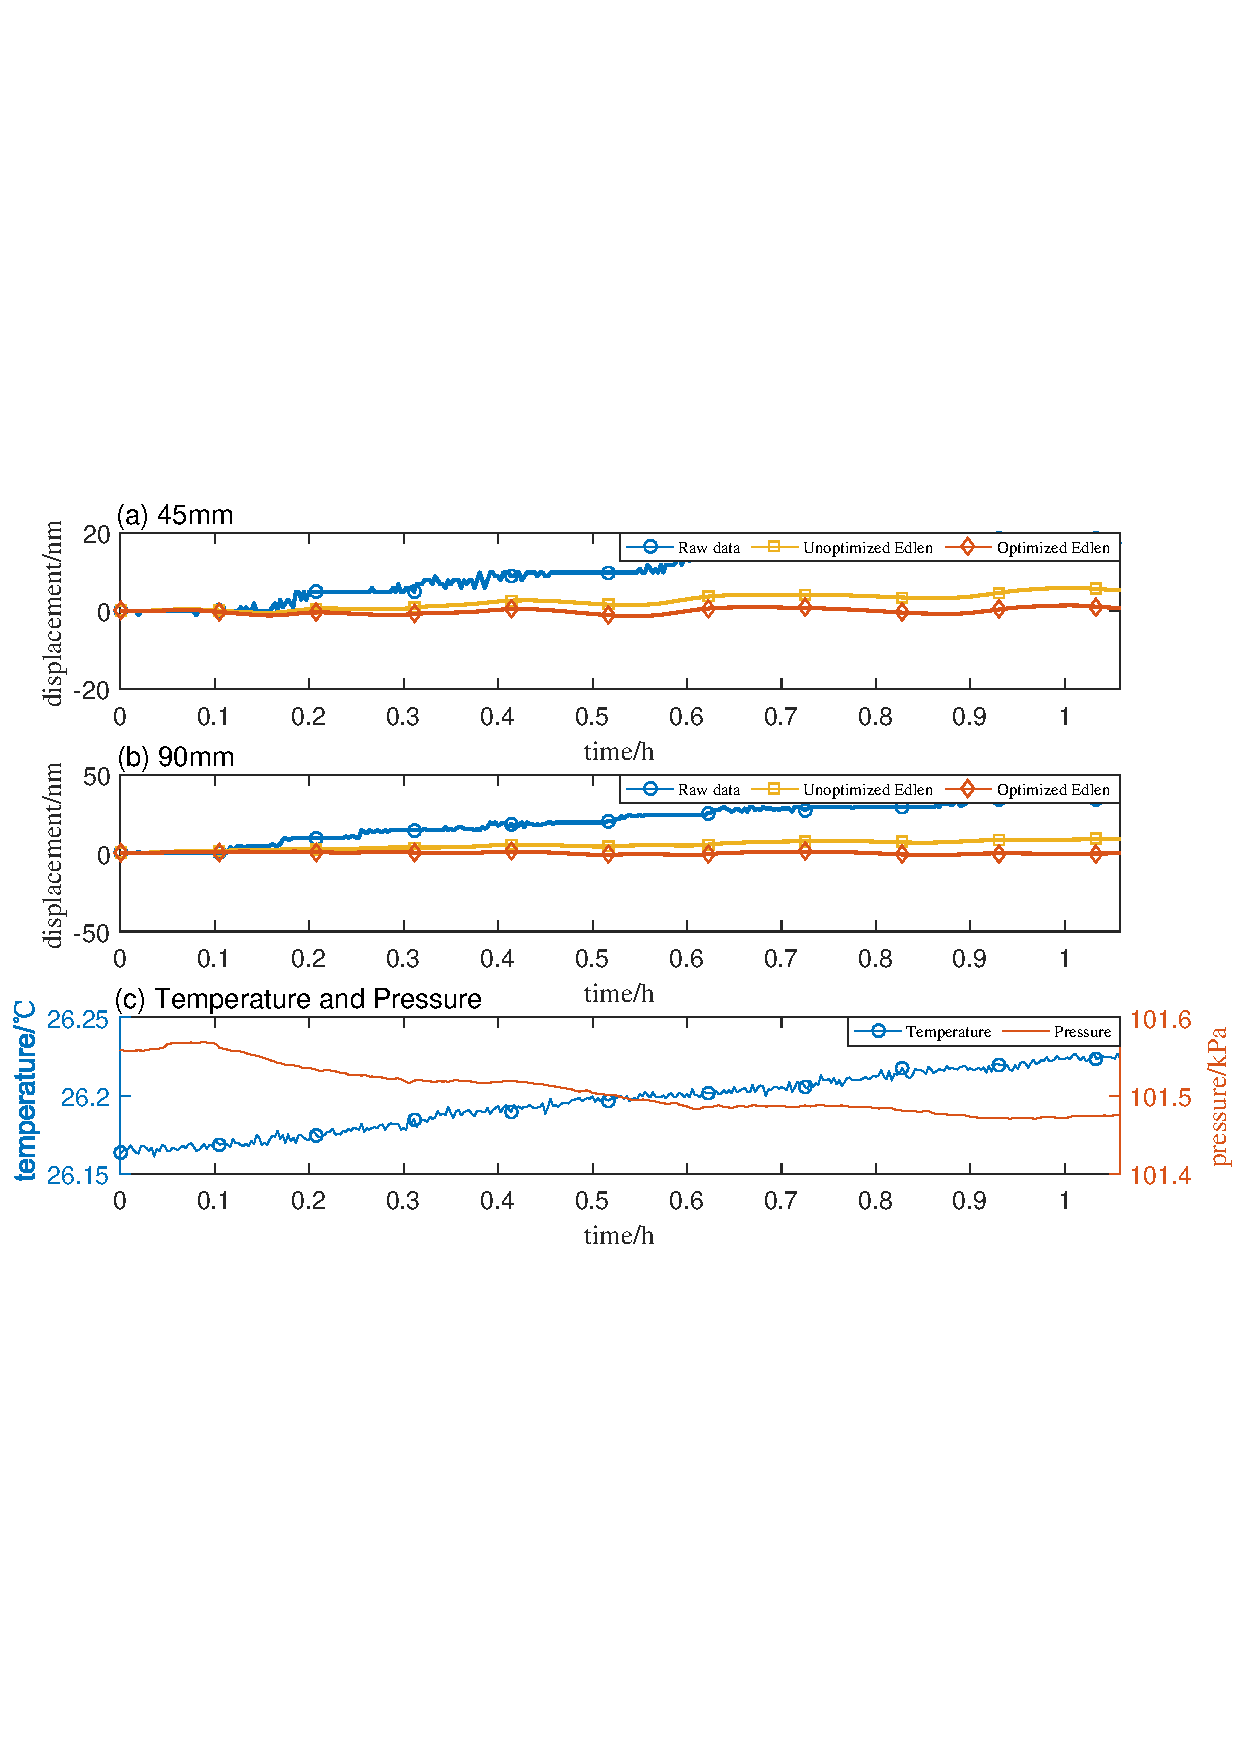
\includegraphics[width=14cm]{fig/4-fig/edpso_短时测量实验数据.pdf}
    \caption{粒子群算法优化后的短时测量补偿效果}
    \label{fig:粒子群算法优化后的短时测量补偿效果}
\end{figure}

如图\ref{fig:粒子群算法优化后的短时测量补偿效果}所示,优化后的红色曲线相比于未经优化的黄色曲线,无论是$45nm$还是$90nm$情况下,都更加接近于理论位移值$0nm$,这说明使用粒子群算法对Edlen公式进行优化之后在进行补偿可以比较明显地提升补偿效果。从数据层面分析,使用粒子群算法进行优化之后再进行补偿,测量臂长度为$45nm$的干涉仪的残留均方根误差从$3.1377nm$降低为$0.8541nm$,而$90nm$长度的则从$5.8401nm$降低为$1.034nm$,分别同比减小了$72.7\%$和$82.3\%$,并且两者残差的差值只有$0.1799nm$,相较于未优化前的差值$2.7024nm$有着较大提升,可以认为使用经过粒子群算法优化之后的Edlen公式进行补偿后的残差在不同测量臂长度情况下是近似相等的,这说明环境误差得到了比较精准并且完全的补偿。但是如果从百分比的角度分析,$0.1799nm$的残差差值占原始残差的比例约为$21\%$,这是一个比较大的百分比,可能的原因是由于改组温度变化较小,使得环境误差在总体误差中的比例不够大。

\subsection{长时测量}
对前文所述的长时测量的实验数据也是用粒子群算法优化后再进行补偿,结果如图\ref{fig:粒子群算法优化后的长时测量补偿效果}所示,虽然采样时长增加了,但是粒子群算法的优化效果依旧显著。从数据层面分析,使用粒子群算法进行优化之后再进行补偿,测量臂长度为$45nm$的干涉仪的残留均方根误差从$14.9957nm$降低为$6.8308 nm$,而$90nm$长度的则从$43.5806nm$降低为$3.6700nm$,两者残差的差值只有$3.16nm$,相较于未优化前的差值$28.5849nm$有着较大提升,可以认为使用经过粒子群算法优化之后的Edlen公式进行补偿后的残差在不同测量臂长度情况下是近似相等的,这说明环境误差得到了比较精准并且完全的补偿。
\begin{figure}[htb]
  \centering
  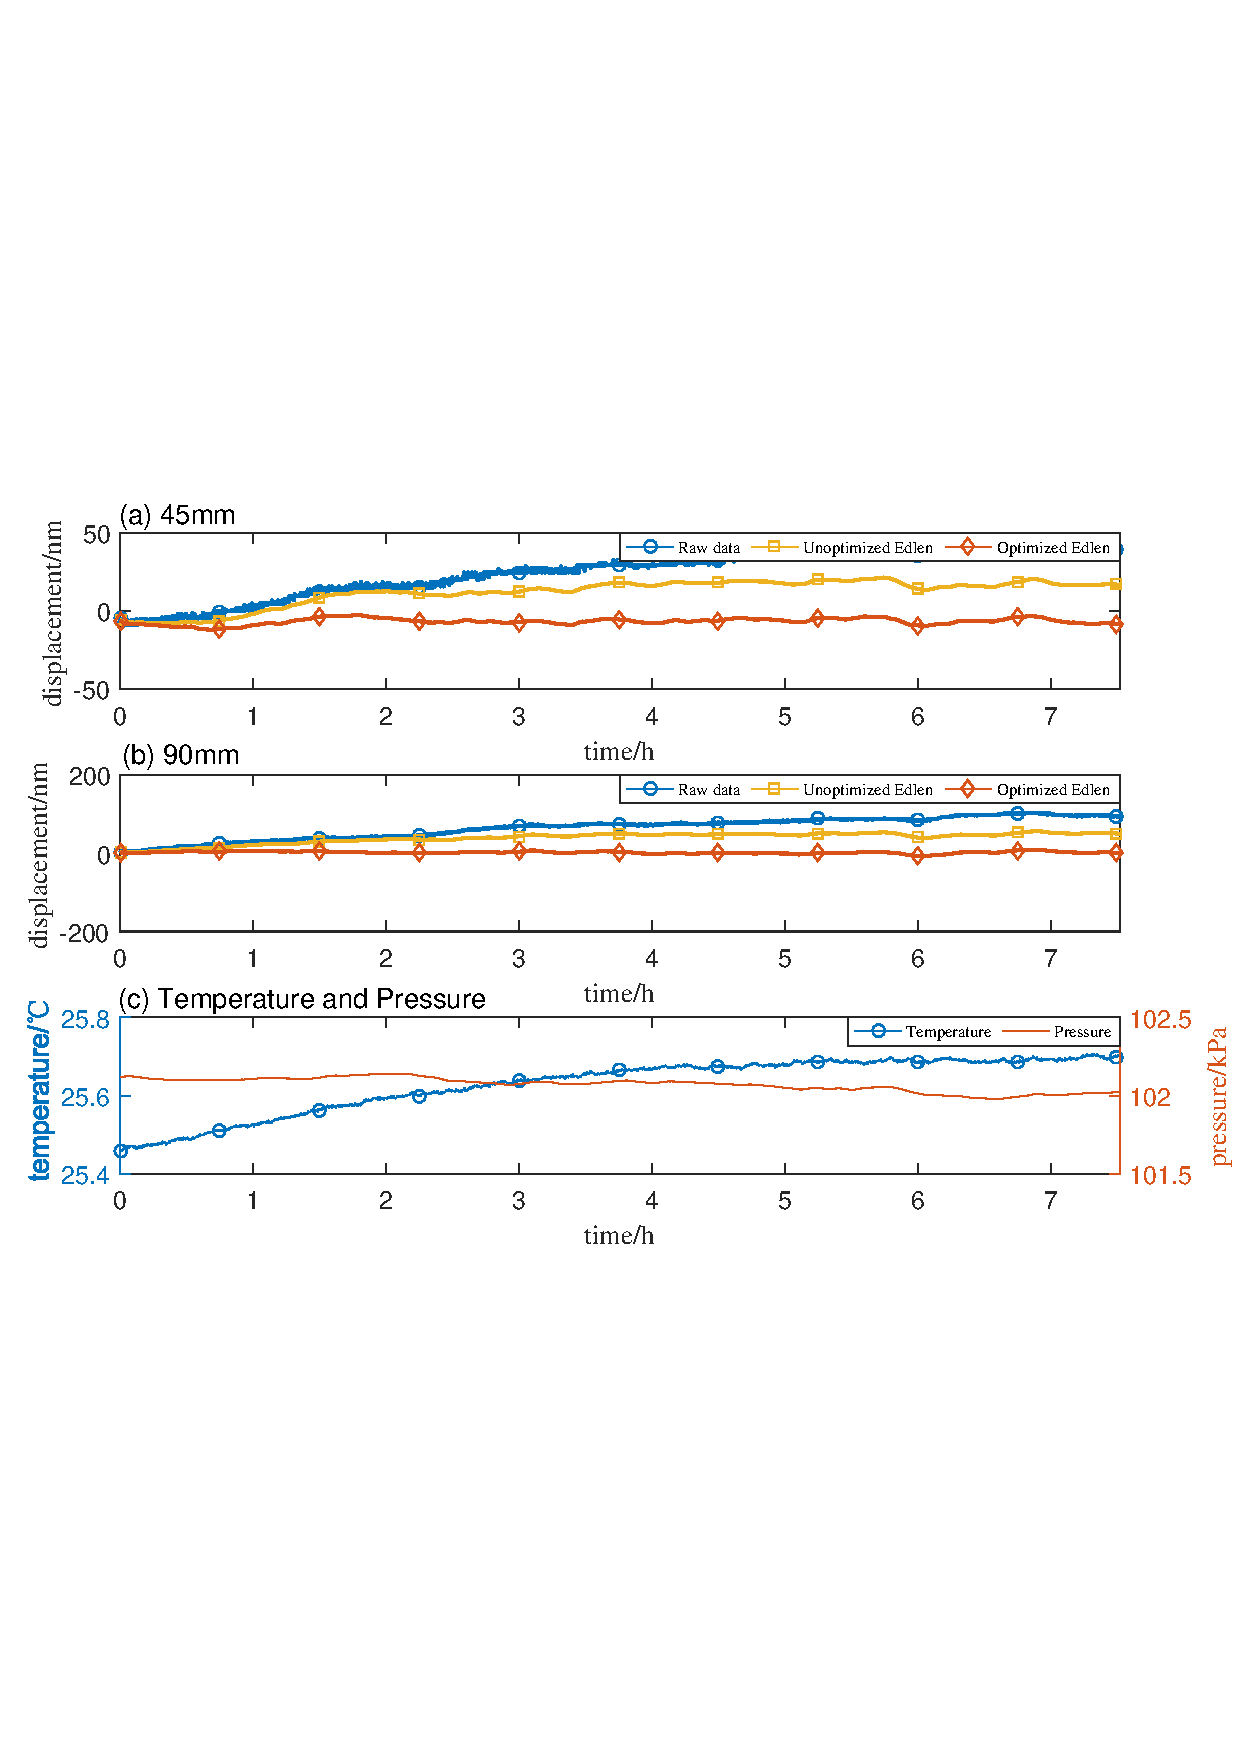
\includegraphics[width=14cm]{fig/4-fig/edpso_长时测量实验数据.pdf}
  \caption{粒子群算法优化后的长时测量补偿效果}
  \label{fig:粒子群算法优化后的长时测量补偿效果}
\end{figure}

同时,从数据中可以发现,测量臂长度为$90nm$的数据经过粒子群算法优化后的补偿残差$3.6700nm$是小于$45nm$的$6.8308nm$,可能原因有:
\begin{enumerate}
  \item 由于粒子群算法在训练过程中使用的是$90nm$的测量数据,并且该组试验的测量时间较长,使得粒子群算法较好地挖掘了数据中潜在的规律,达到比较完美的补偿效果。
  \item $45nm$的测量数据发生了过补偿。
  \item 由于环境补偿后的残差较小,所以可能由于随机误差的干扰。
\end{enumerate}

需要特别说明的是,从其他未给出的实验数据以及下文给出的大范围温度变化测量的结果分析,比较大的可能是由于随机误差的干扰。
\subsection{大范围温度变化测量}
对前文所述的大范围温度变化测量的实验数据也是用粒子群算法优化后再进行补偿,结果如图\ref{fig:粒子群算法优化后的大范围温度变化测量补偿效果}所示,虽然采样时长以及温度变化范围都增加了,但是粒子群算法的优化效果依旧显著。从数据层面分析,使用粒子群算法进行优化之后再进行补偿,测量臂长度为$45nm$的干涉仪的残留均方根误差从$153.6245nm$降低为$29.3458 nm$,而$90nm$长度的则从$176.6071nm$降低为$48.4996nm$,两者残差的差值仍有$19.1538nm$,相较于未优化前的差值$28.5849nm$有着一定提升,这说明环境误差的补偿效果得到一定改善,但是不同测量臂长度下的残差仍然不可以认为是相等的,说明该组实验数据哪怕经过整段式粒子群算法的优化,其补偿效果也只是提升了,并未像前两组实验数据那样得到精准且完全的补偿。
\begin{figure}[htb]
  \centering
  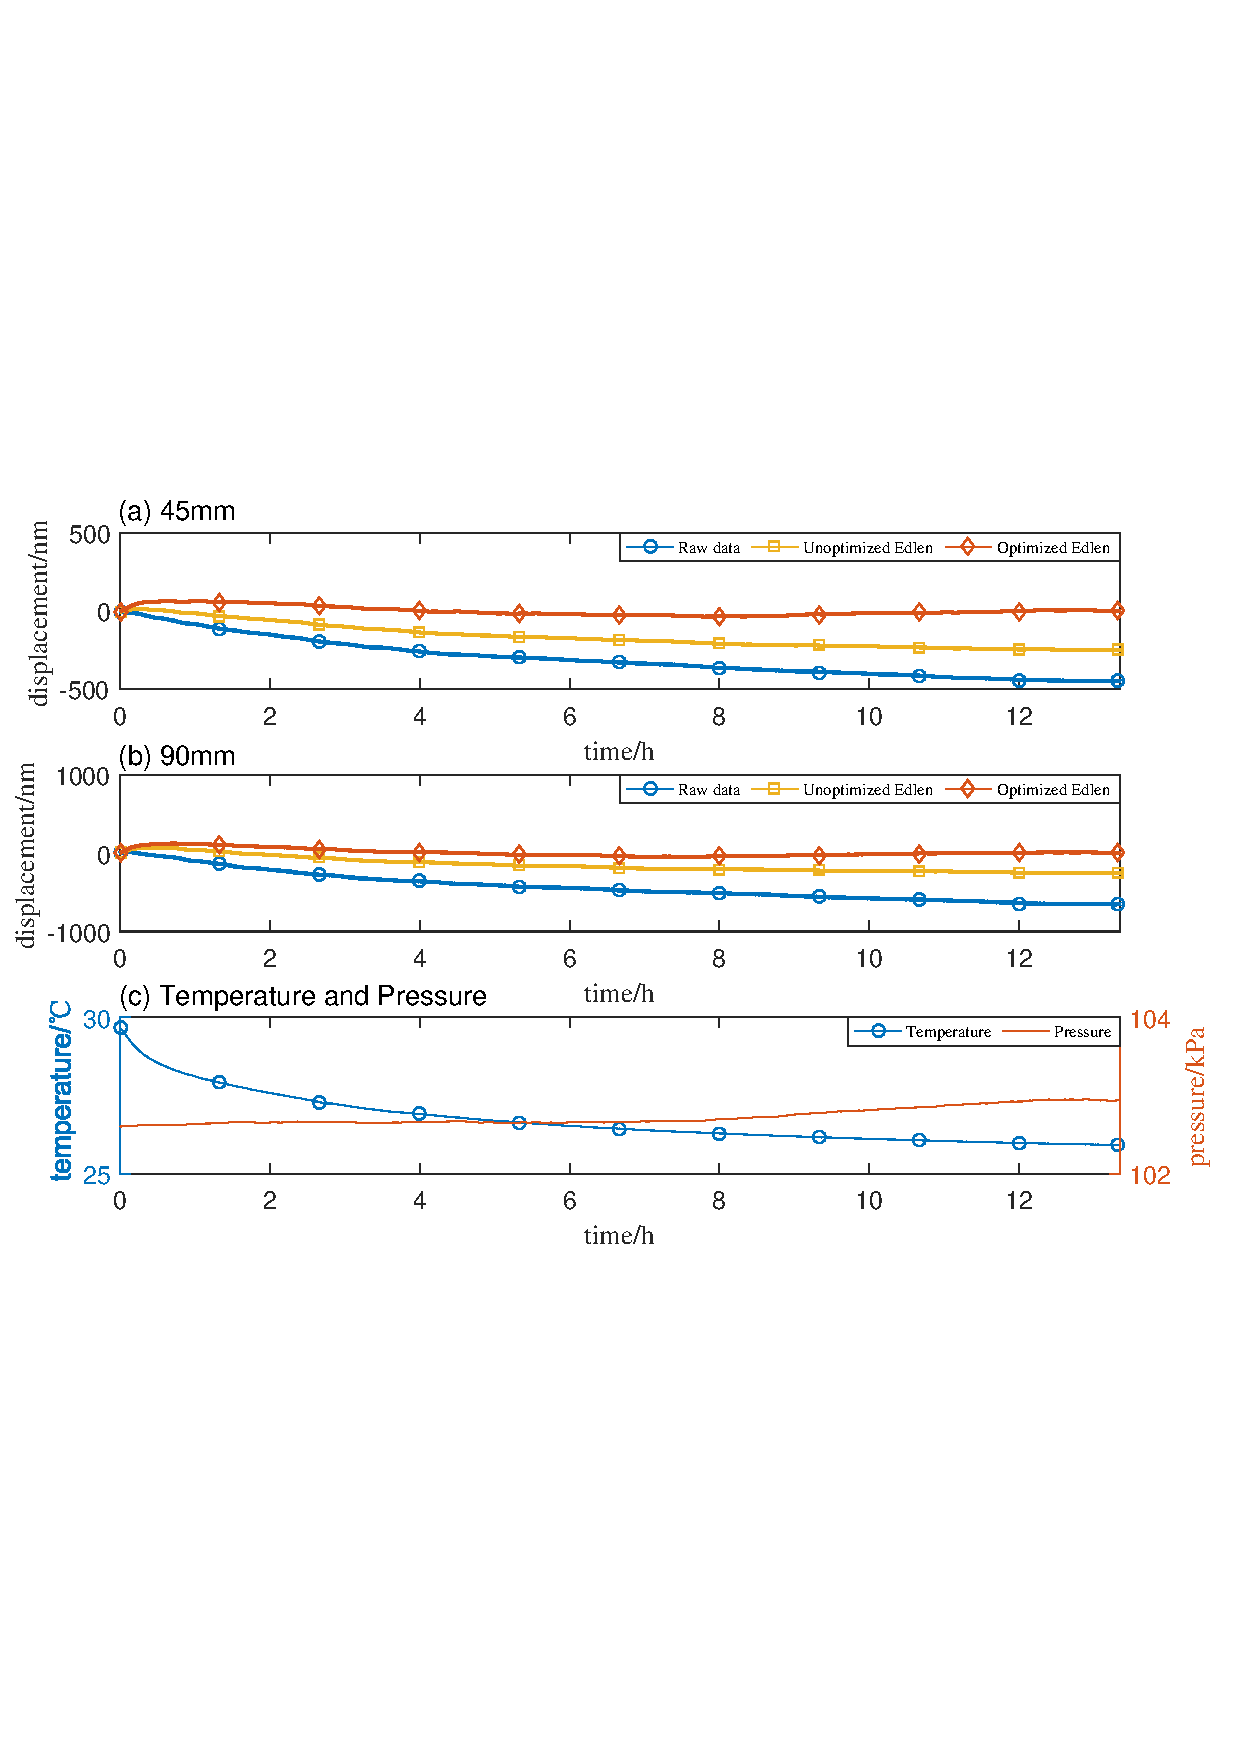
\includegraphics[width=14cm]{fig/4-fig/edpso_大范围温度变化测量数据.pdf}
  \caption{粒子群算法优化后的大范围温度变化测量补偿效果}
  \label{fig:粒子群算法优化后的大范围温度变化测量补偿效果}
\end{figure}

但是从上述的分析数据中可以看出,该组的温度变化以及测量时间均比长时测量实验中长,但是经过粒子群算法优化后再进行补偿得到的残差值,并未出现长时测量实验中:测量臂长度为$45nm$的补偿残差大于测量臂长度为$90nm$的补偿残差,这进一步验证了长时测量实验中出现该现象的原因是由于偶然的随机误差,难以复现。

前$0.8h$时间内的过补偿现象变得更严重了,经粒子群算法优化后的补偿结果的凸起高度从$70nm$增大到了约$120nm$,但是使用粒子群算法优化后在整个$12.5h$测量时间内的补偿效果是改善的,这说明粒子群算法已经比较完全地挖掘出了Edlen公式的补偿性能,只是在大温度梯度的情况下,可能引入了其他误差因素,导致线性形式的Edlen公式无法适用。

\subsection{优越性}
上述的实验结果可以说明,将Edlen公式与粒子群算法相结合,可以比较有效地减小Edlen公式本身温度不匹配、波长不匹配的问题,提高补偿效果。但在\ref{粒子群算法}节中也说明了,将Edlen公式与粒子群算法相结合,也可以很有效地避免粒子群算法自身早熟收敛的问题。如图\ref{fig:粒子群算法训练过程}所示,图\ref{fig:以Edlen公式为起点的训练过程}为以Edlen公式为搜索起点的三次训练过程数据,而图\ref{fig:以零点为起点的训练过程}为以零点为搜索起点的三次训练过程数据,最大迭代次数均为150次。可以明显看出,若以Edlen公式为搜索起点,三次训练结果都能准确落在同一位置,对应的适应度为0.06861,可以认为是找到了全局最优解;而若从零点开始搜索,三次训练结果落在了三个不同位置,对应的适应度分别为0.07031、0.06861、0.08587,只有一次找到了全局最优解,而另外两次都只找到了局部最优解,并且最少又经历了40次迭代都没有跳出这个局部最优解,发生了早熟收敛现象。

\begin{figure}[htb]
  \centering
  \subfigure[以Edlen公式为起点的训练过程]{
    \begin{minipage}[b]{0.99\textwidth}
      \centering
      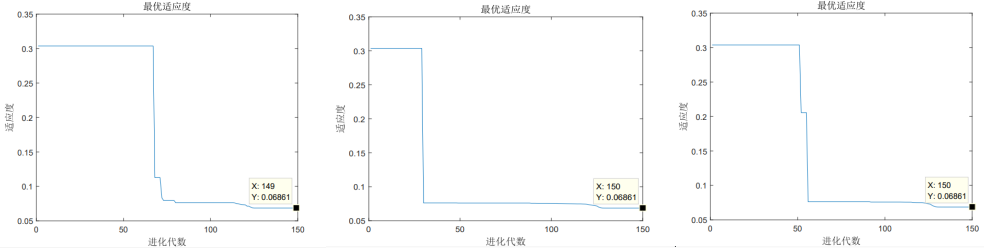
\includegraphics[width=14cm,height=5cm]{fig/4-fig/训练过程a.png}
    \end{minipage}
    \label{fig:以Edlen公式为起点的训练过程}
  }
  \subfigure[以零点为起点的训练过程]{
    \begin{minipage}[b]{0.99\textwidth}
      \centering
      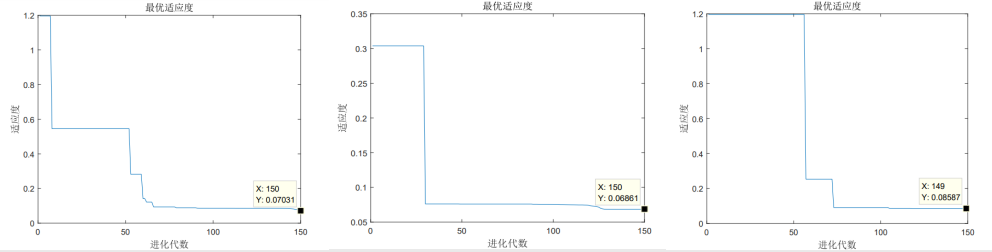
\includegraphics[width=14cm,height=5cm]{fig/4-fig/训练过程b.png}
    \end{minipage}
    \label{fig:以零点为起点的训练过程}
  }
  \caption{粒子群算法训练过程}
  \label{fig:粒子群算法训练过程}
\end{figure}

\subsection{局限性}
为了探究温度梯度对Edlen公式补偿效果的影响,使得温度在$25.64^{\circ}C\sim28.85^{\circ}C$范围内来回变化,并使用原始Edlen公式以及经粒子群算法优化后的Edlen公式对其进行补偿,实验结果如图\ref{fig:温度梯度实验数据}所示。
\begin{figure}[htb]
  \centering
  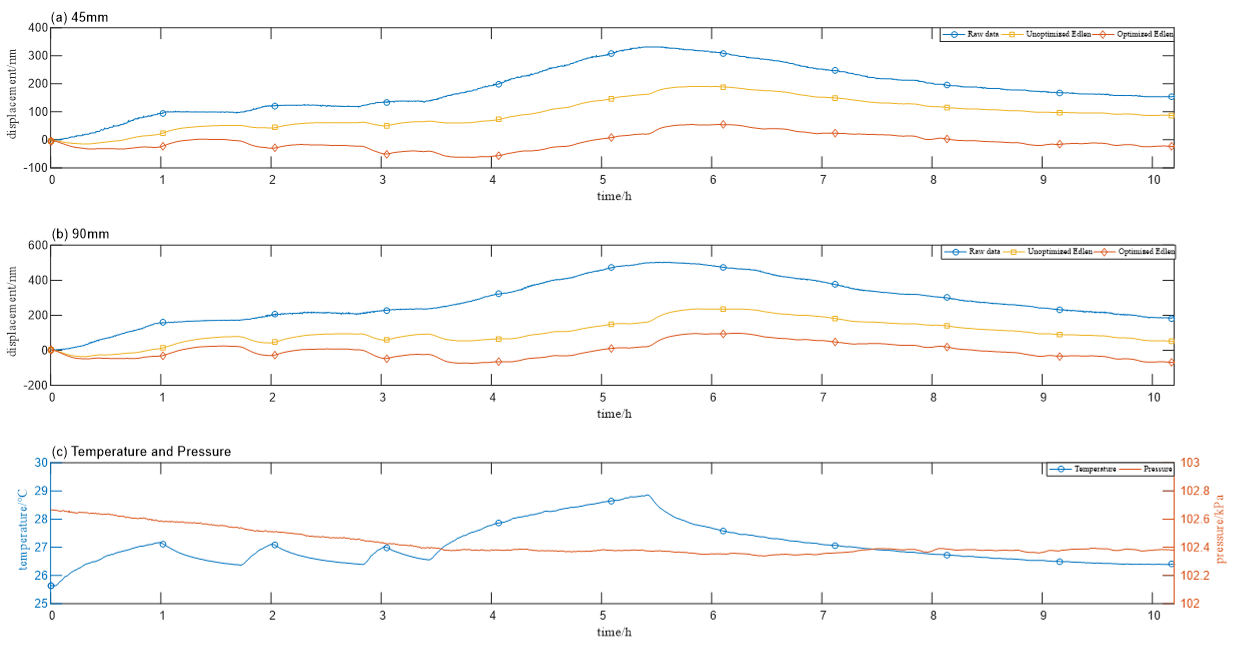
\includegraphics[width=14cm]{fig/4-fig/温度梯度实验数据.jpg}
  \caption{温度梯度实验数据}
  \label{fig:温度梯度实验数据}
\end{figure}

测量时间约为$10.2h$,温度变化范围为$[25.64\,\,\,28.85]^{\circ}C$,气压变化范围为$[102.7\,\,\,102.4]kPa$,测量臂长度为$45nm$和$90nm$的两套干涉仪的原始位移数据的变化范围为$[0 \,\,\, 301.3]nm$和$[0\,\,\,582.4]nm$,在考虑可能含有随机误差等其他误差的情况下,可近似认为两者成两倍关系。并且对于零位测量而言,上述位移变化都可以认为是误差,对应的均方根误差分别为$201.8186nm$和$379.4892nm$。经过Edlen公式补偿后的均方根误差为$108.9044nm$和$124.7847nm$,补偿效果约为$46\%$和$67\%$。使用粒子群算法进行优化之后再进行补偿,测量臂长度为$45nm$的干涉仪的残留均方根误差从$108.9044nm$降低为$30.4053 nm$,而$90nm$长度的则从$124.7847nm$降低为$45.8778nm$,两者残差的差值仍有$15.4725nm$,相较于未优化前的差值$15.8803nm$几乎没有提升,这说明这说明环境误差的补偿效果得到一定改善,但补偿的精准性却不一定有提升。

从图中可以看出,$1\sim2h$、$2\sim3h$时间内,温度在$26^{\circ}C\sim27^{\circ}C$范围内来回变化,在$3.4\sim10h$内,温度则从$26^{\circ}C$上升到$28.85^{\circ}C$,随后又回到$26^{\circ}C$,前两次的温度梯度明显大于最后一次的温度梯度。从补偿结果也可以看出,红色曲线为经过粒子群算法优化后的Edlen公式的补偿效果,相较于原始Edlen公式的补偿效果(黄色曲线),红色曲线明显更加贴近理论位移值0nm。但黄色曲线以及红色曲线在上述三个温度波动范围也有明显波动,并且第三个温度波动范围内对应的补偿结果波动较前面两个显得更加平缓,与温度梯度值的大小相对应。这进一步说明了,在大温度梯度的情况下,可能引入了其他误差因素,导致线性形式的Edlen公式无法适用。

\section{基于温度梯度的分段式粒子群算法补偿方法}
\subsection{算法原理}
由前文所述可知,在大温度梯度的情况下,可能引入了其他误差因素(例如大气湍流),导致线性形式的Edlen公式无法适用,此时的补偿模型可能是非线性的。但是由微积分的思想可知,一个非线性的函数只要微分的粒度足够小,在每一个$\Delta t$区间内都可以看做是线性的。所以只需要进行分段,然后在各个微分段内,Edlen公式仍是可以使用的。由于温度梯度才是导致上述问题的原因,那么在进行分段补偿的时候,自然使用温度梯度作为分段的依据,在本文所述的工作中,采用如下两种分段的方法:
\begin{enumerate}
  \item 采用单组温度传感器,使用自身温度的变化梯度作为分组依据,即在一定的时间内,温度的变化超过某个定值就进行一次分段。
  \item 采用两组温度传感器,两组传感器放置的位置具有一定距离,采用同时刻两个传感器的差值作为分组依据,即在同一时刻,两个传感器的差值大于某个定值就进行一次分段。
\end{enumerate}

值得说明的是,在本文进行的实验中,上述两种分段方法的补偿效果差别不大(不超过$3.5\%$),但是第一种方法操作较为简便,所以建议使用第一种方法,本文后续的工作使用的也是第一种方法,使用的阈值为:80个数据点内,温度的变化超过$0.05^{\circ}C$

\subsection{算法流程图}
\label{基于温度梯度的分段式粒子群算法补偿流程图}
算法的流程图如图\ref{fig:基于温度梯度的分段式粒子群算法补偿流程图}所示。
\begin{figure}[htb]
  \centering
  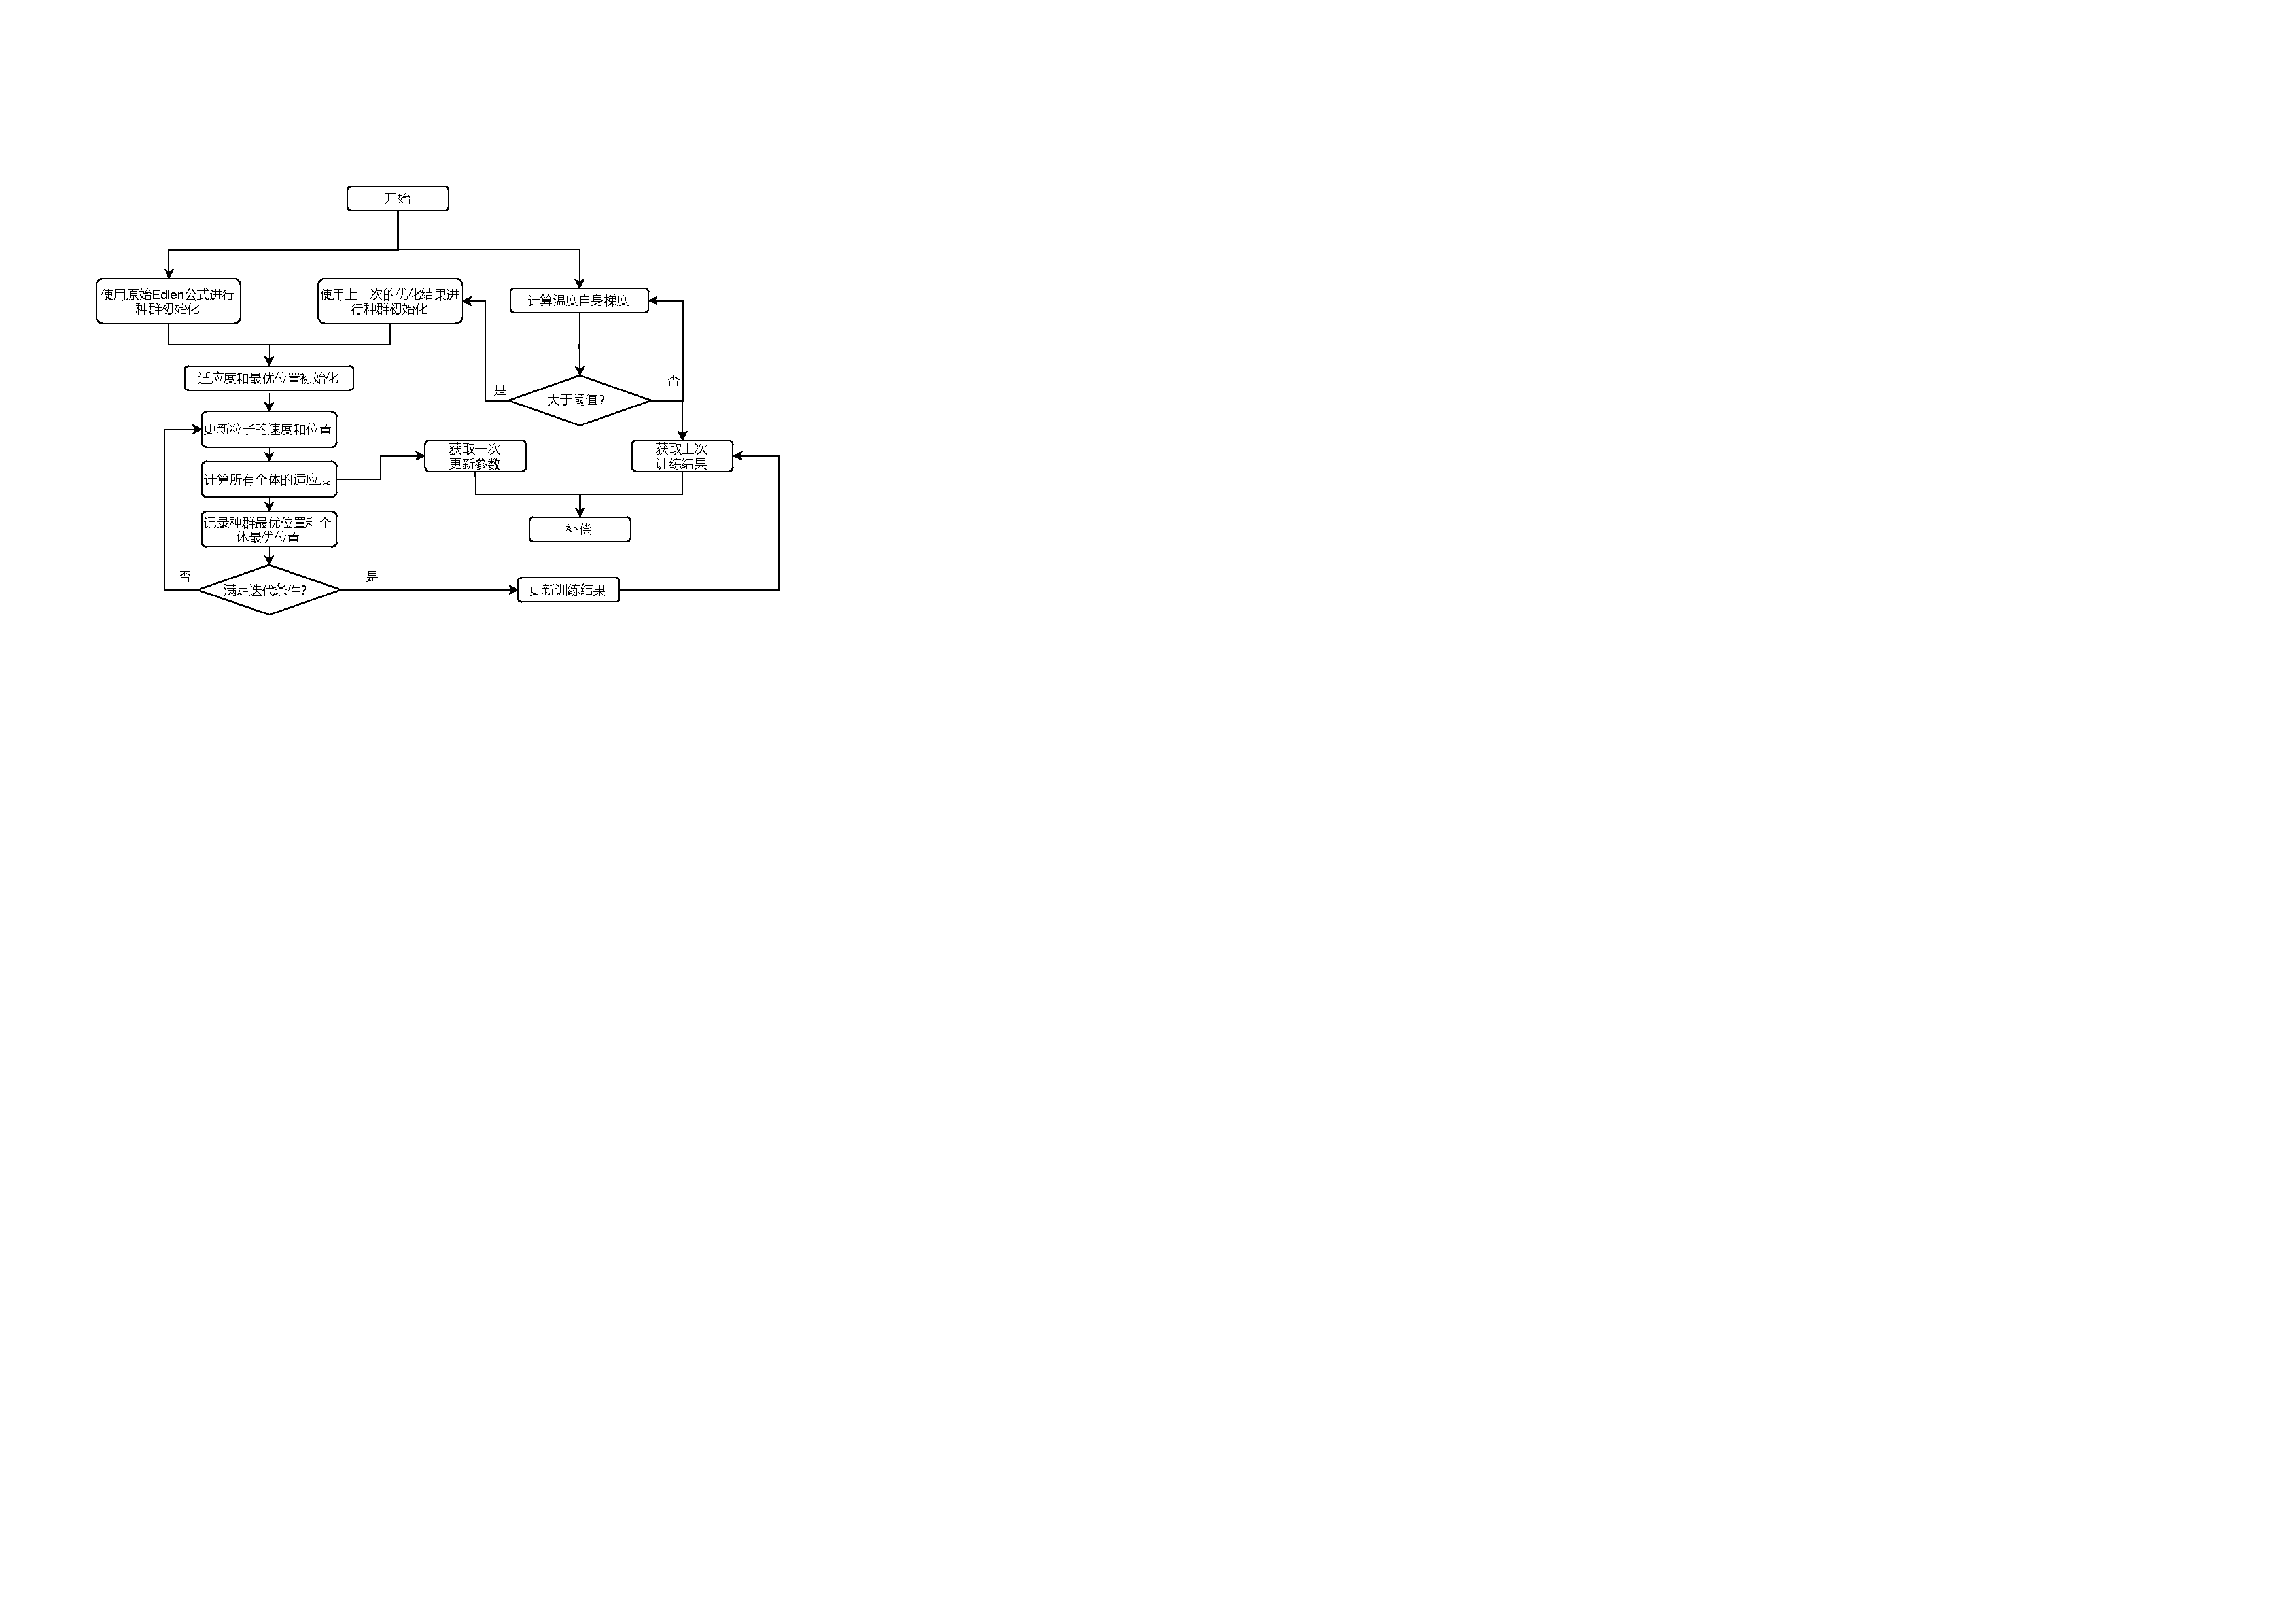
\includegraphics[width=12cm]{fig/4-fig/基于温度梯度的分段式粒子群算法流程图.drawio.pdf}
  \caption{基于温度梯度的分段式粒子群算法补偿流程图}
  \label{fig:基于温度梯度的分段式粒子群算法补偿流程图}
\end{figure}

跟之前介绍的整段式粒子群算法补偿方法不同,当由于温度变化梯度过大导致触发分段进行新的一次粒子群算法训练时,种群的初始不再是设置为原始的Edlen公式,而是设置为触发分段之前的粒子群算法的训练结果,这就意味着在进行新的一次分段训练的前期,进行补偿的Edlen公式模型并不是粒子群算法训练出来的最优解,而是一个更上一次训练结果比较接近的次优解,这么做是为了让补偿结果的曲线比较平滑,防止在两次分段训练的交界处,由于补偿模型的突然改变而使得补偿结果曲线出现突然的断落。但由于使用了一个次优解而非最优解,势必会对补偿精度造成一定损失,损失的大小取决于采样周期与粒子群算法计算速度之间的关系。采样周期越长,粒子群算法计算速度越快,那么在进行新的一次分段补偿时,能够给粒子群算法训练的时间也就越多,训练效果也就越好,精度损失也就越小,反之亦然。由于温度梯度改变可能会导致触发新的一次分段训练,但当前训练的迭代次数可能还没达到设置的迭代上限就开始了新的一轮训练,从而使得上轮训练不彻底。所以迭代条件不能简单用迭代次数进行控制,为此增加了使用适应度大小进行控制,即迭代次数到达上限或者适应度小于设定的阈值,视为完成一轮迭代。

\subsection{补偿效果}
实验数据如图\ref{fig:基于温度梯度的分段粒子群算法补偿效果}所示。(a)图为测量臂长度为$45nm$的位移测量数据,(b)图为测量臂长度为$90nm$的位移测量数据,(c)图为对应的温度和气压数据,(a)、(b)、(c)三图的横轴均为时间,单位为h;(a)和(b)图中的竖轴为位移数据,单位为$nm$,其中带圆圈标注的蓝色曲线为原始的位移测量数据,带黄色方块标注的为使用原始Edlen公式补偿后的位移数据,带红色菱形标注的为使用粒子群算法优化后的补偿后位移数据,带五角星形标注的则为基于温度梯度的分段粒子群算法补偿后的位移数据;(c)图的竖轴为温度和气压数据,单位为$^{\circ}C$和$kPa$,其中带圆圈标注的蓝色曲线为温度数据,红色曲线为气压数据。

\begin{figure}[htb]
  \centering
  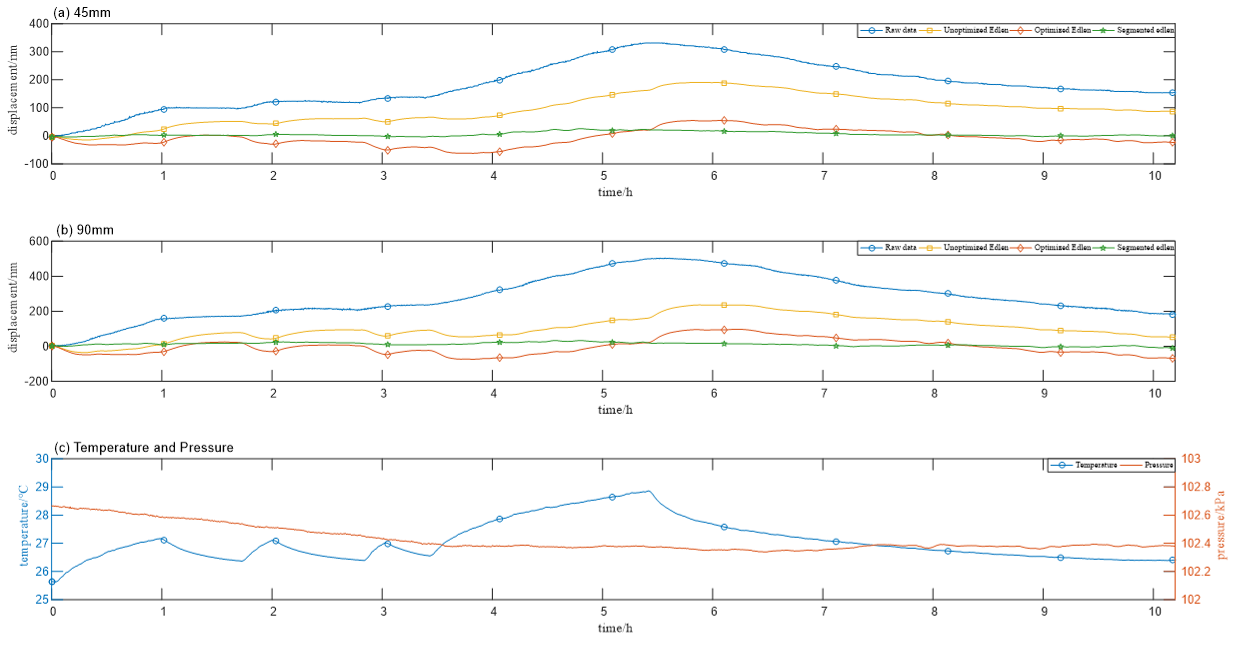
\includegraphics[width=14cm]{fig/4-fig/基于温度梯度的分段粒子群算法补偿效果.jpg}
  \caption{基于温度梯度的分段粒子群算法补偿效果}
  \label{fig:基于温度梯度的分段粒子群算法补偿效果}
\end{figure}

数据上,相比经过整段式粒子群算法的补偿效果,在经过E温度梯度的分段粒子群算法补偿后的均方根误差从$30.4053 nm$降低到了$10.7903 nm$($45nm$)、从$45.8778 nm$降低到了$13.1134 nm$($90nm$),剩余的残差也仅仅只有$2.3631nm$,这个数值甚至小于干涉仪的分辨率,所以完全可以认为补偿后的残差是相等的,即可以说明环境误差得到了比较精确且完全的补偿。图形上也可以看出,绿色的线几乎全程保持一条直线,并没有过大的波动。

\subsection{不足之处}
需要特别指出的是,基于温度梯度的分段式粒子群算法补偿方法仍然有着以下几个不足之处:
\begin{enumerate}
  \item 进行分段时所使用的依据:80个数据点内,温度的变化超过$0.05^{\circ}C$也是一个经验值,是根据本文工作的实验数据分析出的一个补偿效果比较理想的值,这就意味着也可能存在上文所述的诸如温度不匹配或其他类似问题,这可能也会一定程度上影响补偿效果。
  \item 如\ref{section:实验环境改进}节所述,本文的所有工作都未在亚克力罩中设置任何的直接热源,温度梯度的值无法做到太大,这就导致了未验证过当温度梯度进一步增大时,基于温度梯度的分段式粒子群算法补偿方法的效果如何。
  \item 如\ref{基于温度梯度的分段式粒子群算法补偿流程图}节所述,采样周期越长,粒子群算法计算速度越快,两者之间的差值越大,那么在每次分段补偿的初期补偿效果损失越小。但是当前干涉仪的应用场合下,大多无法做到过低的采样频率,所以需要想办法增加粒子群算法计算速度。
  \item 如\ref{基于温度梯度的分段式粒子群算法补偿流程图}节所述,可能会出现当前训练的迭代次数可能还没达到设置的迭代上限就开始了新的一轮训练的情况,虽然使用适应度控制迭代条件能减少该情况的发生,但是适应度阈值的取值也有着一定的要求,适应度阈值过大则仍旧可能会发生上述现象。一般的,在同样的时间内,粒子群算法计算的越快,则迭代计算的结果更优,即适应度更小,需要想办法增加粒子群算法计算速度。
  \item 由于进行了多次分段,这使得整个补偿程序的计算量是明显大于整段式粒子群算法补偿方法的,处于补偿及时性的考虑,计算量增大了需要增加计算速度才能动态平衡。
\end{enumerate}

前两点算是本文工作真正存在的局限性,而后三点的解决办法都相同:提高粒子群算法的计算速度。粒子群算法本质上是一个迭代计算和并行计算相互组合的过程,在达到迭代条件之前需要一直迭代,并且每次迭代需要并行计算每个个体的适应度、更新种群信息、更新个体速度和位置等,其本身计算量就不小。而温度梯度的分段式粒子群算法补偿方法,由于根据温度变化梯度进行分段训练和补偿,将粒子群算法的这一缺点进行了放大。而在当前处理器性能,专用处理器是大于通用处理器的,而粒子群这样一个含有大量并行计算的算法,提升其计算速度的一个有效方法就是设计粒子群算法的专用处理器。

\section{算法硬化}
软件层面和硬件层面的设计是不相同的,软件注重简洁性、高效性,而硬件注重的是面积、功耗、性能三者之前的权衡,所以通常在做硬件实现的时候,都需要对算法做一定更改,使其更加符合硬件设计的逻辑,这步称为算法硬化。硬化后的算法也可以在最后的RTL(Register Transfer Level,寄存器传输级)的参考模型,称为RTL model。

\subsection{数据定点方案及截断方案}
由于在硬件的视角中,只能识别两个电平:0和1,对应的即为二进制数,并且硬件是无法自动识别小数的,当前硬件中表示小数的方案有两种:定点和浮点。定点数指的是约定所有数据都有着一个隐含的小数点,并且这个小数点位置是固定的,例如8bit的数据(bit7-bit0),bit4和bit3之间为小数点位置,那么高4bit数据(bit7-bit4)则表示整数部分,低4bit数据(bit3-bit0)则表示小数部分,如果是一个有符号数,那么往往在最高位增加1bit(bit8)用来表示正负,如图\ref{fig:定点数示意图}所示,其中1表示负数,0表示正数,例如一个9bit数9'h001011010,由于bit8为0,所以这是一个正数,而bit7-bit4为4'b0101,对应的十进制数为3,所以整数部分为3,而bit3-bit0为4'b1010,对应的十进制数为10,由于这是小数部分,而且是4bit的小数,所以对应的小数精度为$\frac{1}{2^4}$,所以小数部分对应的十进制数为$3+10\times\frac{1}{2^4}=3.625$。浮点数则是指小数点的位置是不固定的,用尾数和阶码表示一个浮点数,其中尾数决定了浮点数的精度并决定了数字的正负,阶码则决定了小数点在数据中的实际位置,科学计数法就是一种常见的浮点数表示方法,例如一个科学计数法表示的数$1.3564\times10^{2}$,其中1.3564则为尾数,它决定了这个数字的精度为0.01;2则为阶码,它决定了小数点的实际位置是在5之后。
\begin{figure}[htb]
  \centering
  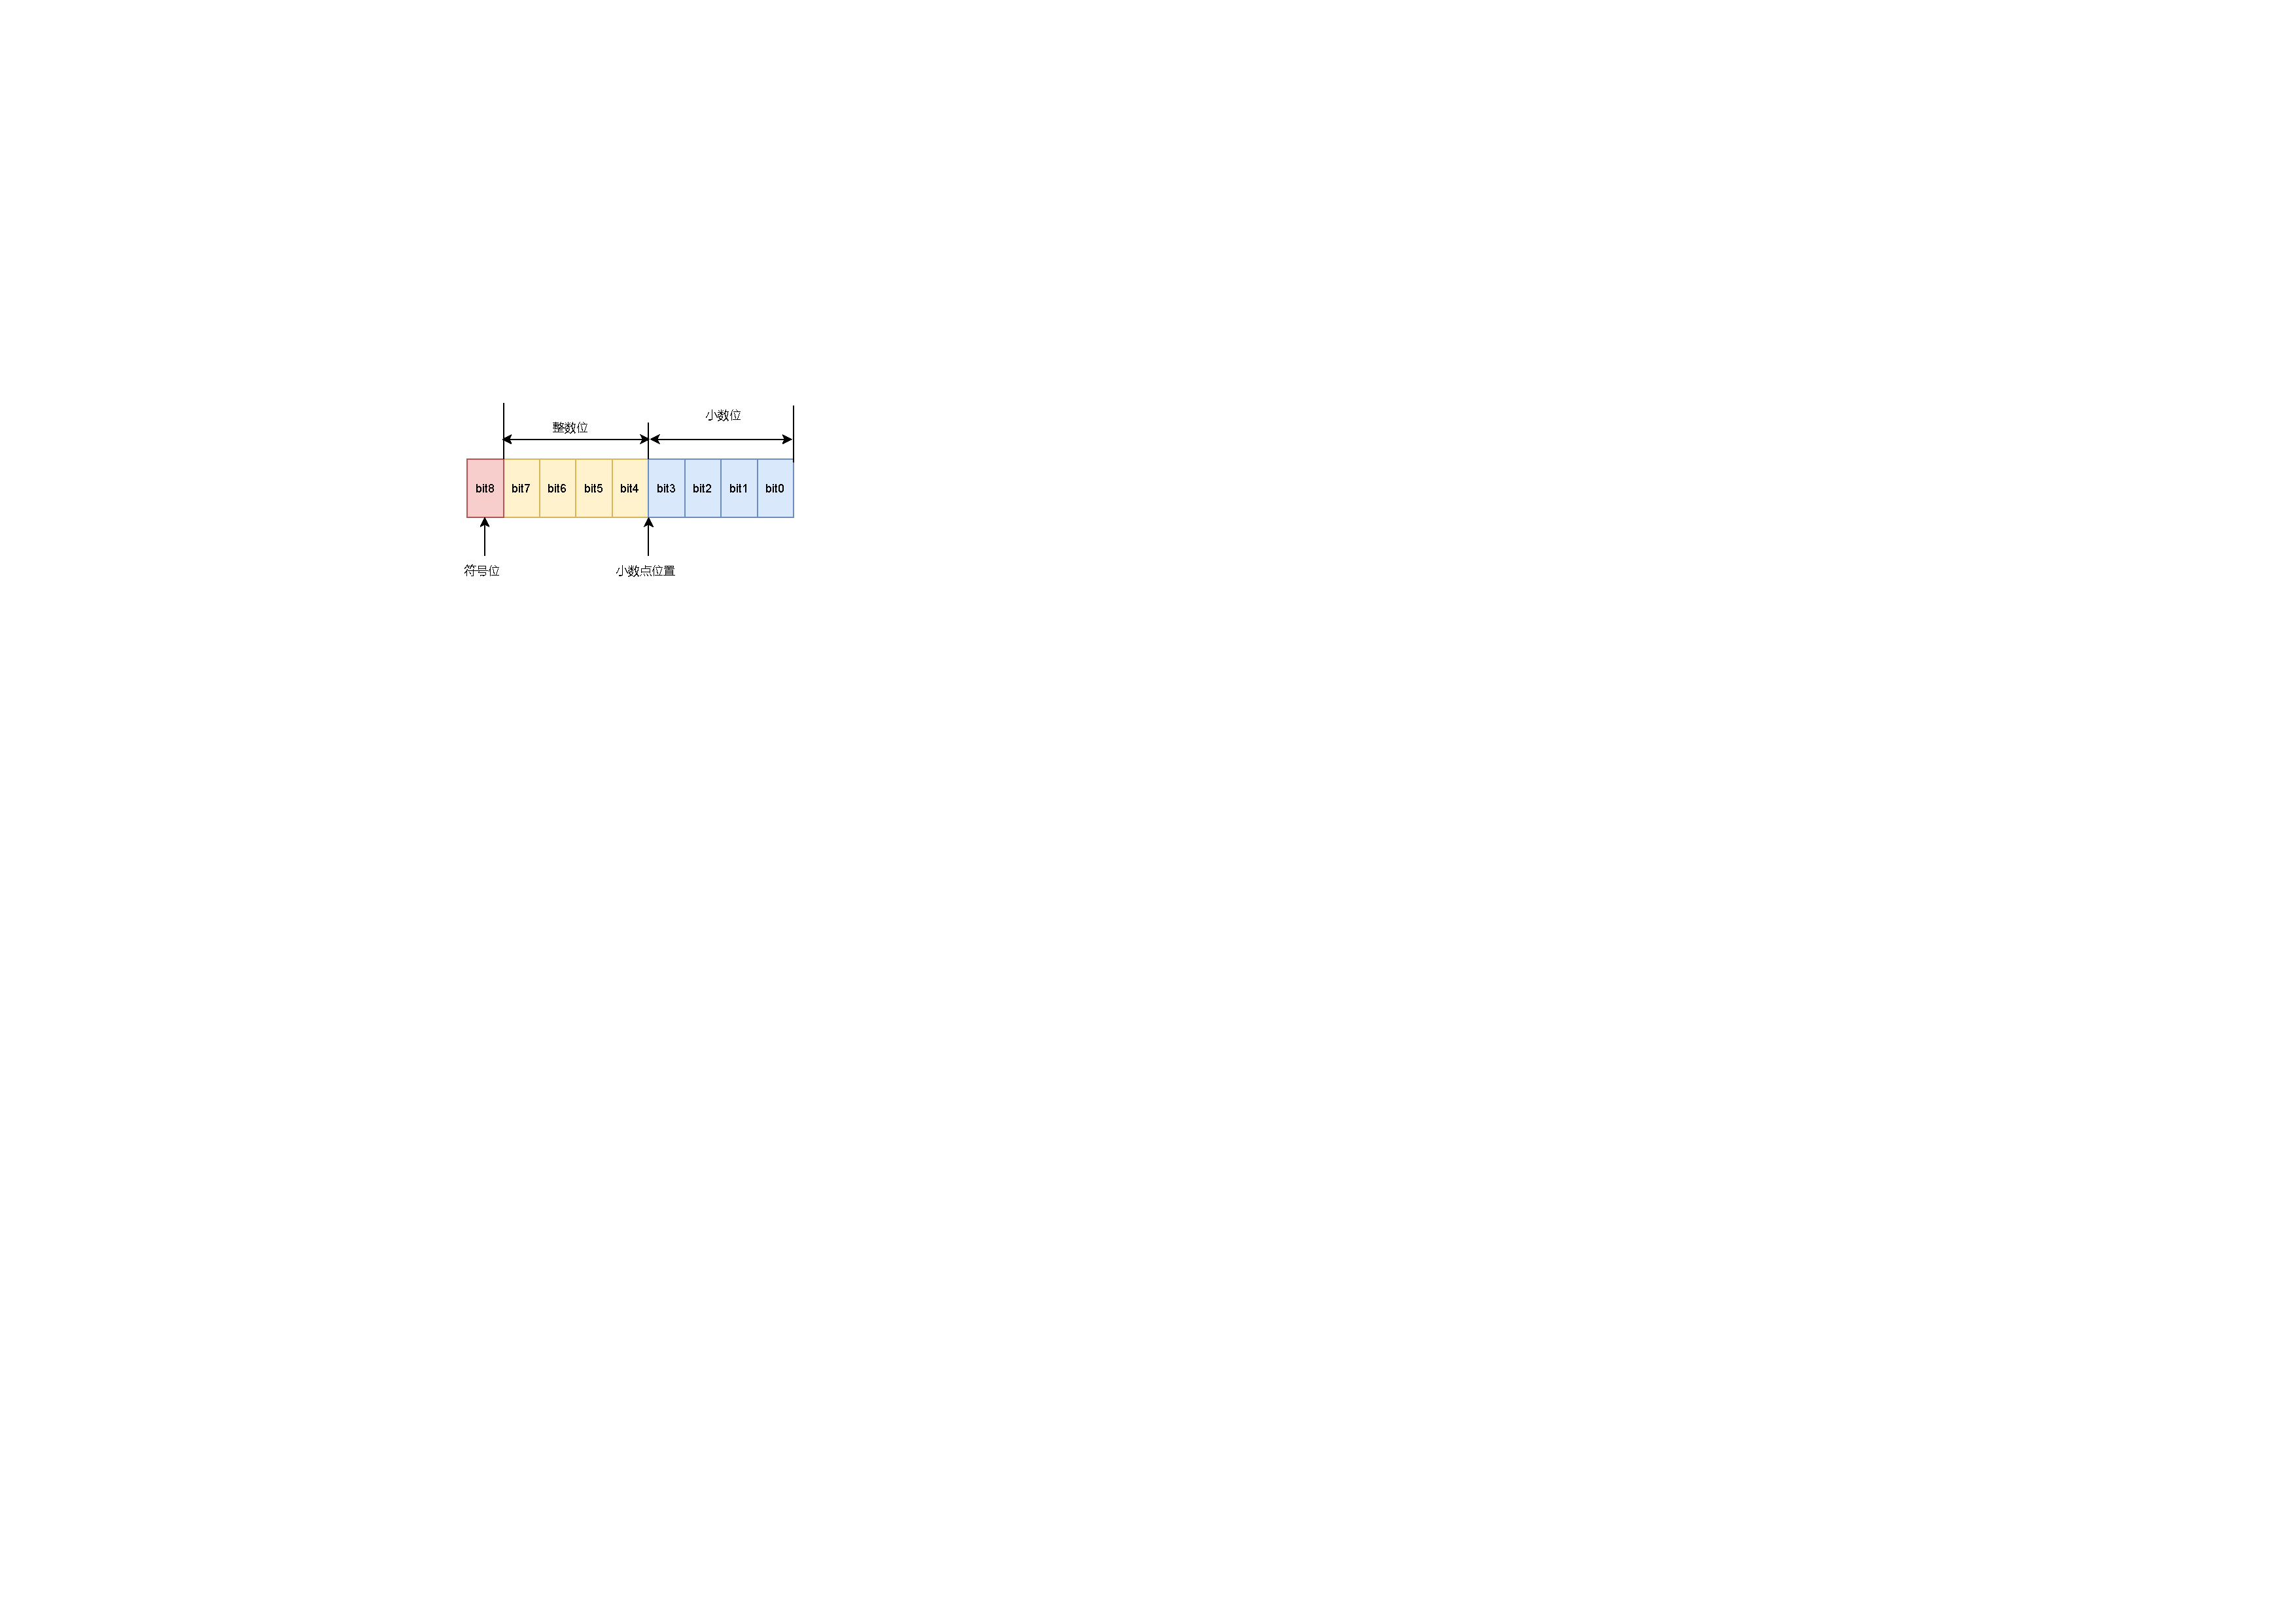
\includegraphics[width=9cm]{fig/4-fig/定点数示意图.drawio.pdf}
  \caption{定点数示意图}
  \label{fig:定点数示意图}
\end{figure}

定点数与浮点数相比,由于小数点的位置是固定的,所以能表示的数值范围也是固定且小于浮点数的表示范围的,这导致可能会存在数值溢出的问题,但是定点数有着一个最大的优点:定点数对应的计算单元运算更快,并且消耗更少的资源和功率,所以为了提高粒子群算法的计算速度,定点数是比浮点数更好的选择。

所以本文采用1bit符号位加上15bit整数加上8bit小数共24bit的定点方案,小数部分最大截断误差约为0.0039,该方案能够表示的数据范围约为$-32768nm\sim16384nm$,如果需要表示超过上述范围的数字,需要增加整数部分的比特位宽,想增加数字精度则需要增加小数部分的比特位宽,但这都会带来硬件资源的增加以及性能的下降。

需要注意的是,由于采用了定点方案使得能表示的数值精度是一定的,但是硬件计算加法和乘法的时候,计算结果的比特位宽是会变化,有如下规律:加法结果的数值比特位宽为两个加数之中最大的数值比特位宽+1,乘法结果的数值比特位宽为两个乘数的数值比特位宽之和(注意是数值比特位宽,符号位另作计算),而比特位宽的改变可能会使得在如上所述的24bit定点方案中的精度发生改变,这是错误的,所以实时进行截断。例如两个24bit的定点数相乘,其数值的比特位宽是23bit加1bit的符号位,所以其计算结果是46bit加上1bit的符号位,共计47bit,但是这其中包含了30bit的整数部分和16bit的小数部分,而定点数的精度是一定的,为8bit,经过乘法计算后却增大到了16bit,所以需要将计算结果的最低8bit进行截断。一旦进行了截断就势必会引入误差,而且不同的截断方案引入的误差会是不一样,例如计算$A\times B+C$(A、B、C)均为24bit的定点数,有两种截断方案:计算完$A\times B$后截断和$A\times B+C$全部计算完之后再截断,前者由于计算中途就进行了截断,从而损失了8bit的精度,这会导致误差的累计,但由于少了8bit数,所以可以减少硬件资源的消耗,所以有利有弊。本文综合使用两种截断方案,在需要较高精度的场合,例如适应度计算,采用第二种截断方案以提高计算精度,从而能够比较出适应度非常接近的两个粒子究竟谁更优,而在其余场合则使用第一种截断方案,从而达到节省硬件资源开销的目的。

\subsection{补码运算}
24bit的定点数方案共定义了1bit符号位以及23bit的数值位,对于这样的有符号数,硬件需要区分数据的符号位以及数值位,并且减法器的设计是比加法器更加复杂的,需要更多的硬件资源,所以使用补码将符号位和数值位、加法和减法相统一,这样做能简化硬件层面的设计。

在介绍补码之前需要先简单介绍补码和反码,原码就是指的有符号二进制数本身,而正数的反码也等于它本身,负数的反码则等于其原码除符号位外所有比特位都取反,补码则等于其反码加上1。对于正数而言,原码、反码、补码完全一致,所以实际上原码、反码和补码只对负数具有实际的应用意义。\ref{fig:补码计算示意图}给出了一个8bit有符号数(十进制为-53)的补码计过程。
\begin{figure}[htb]
  \centering
  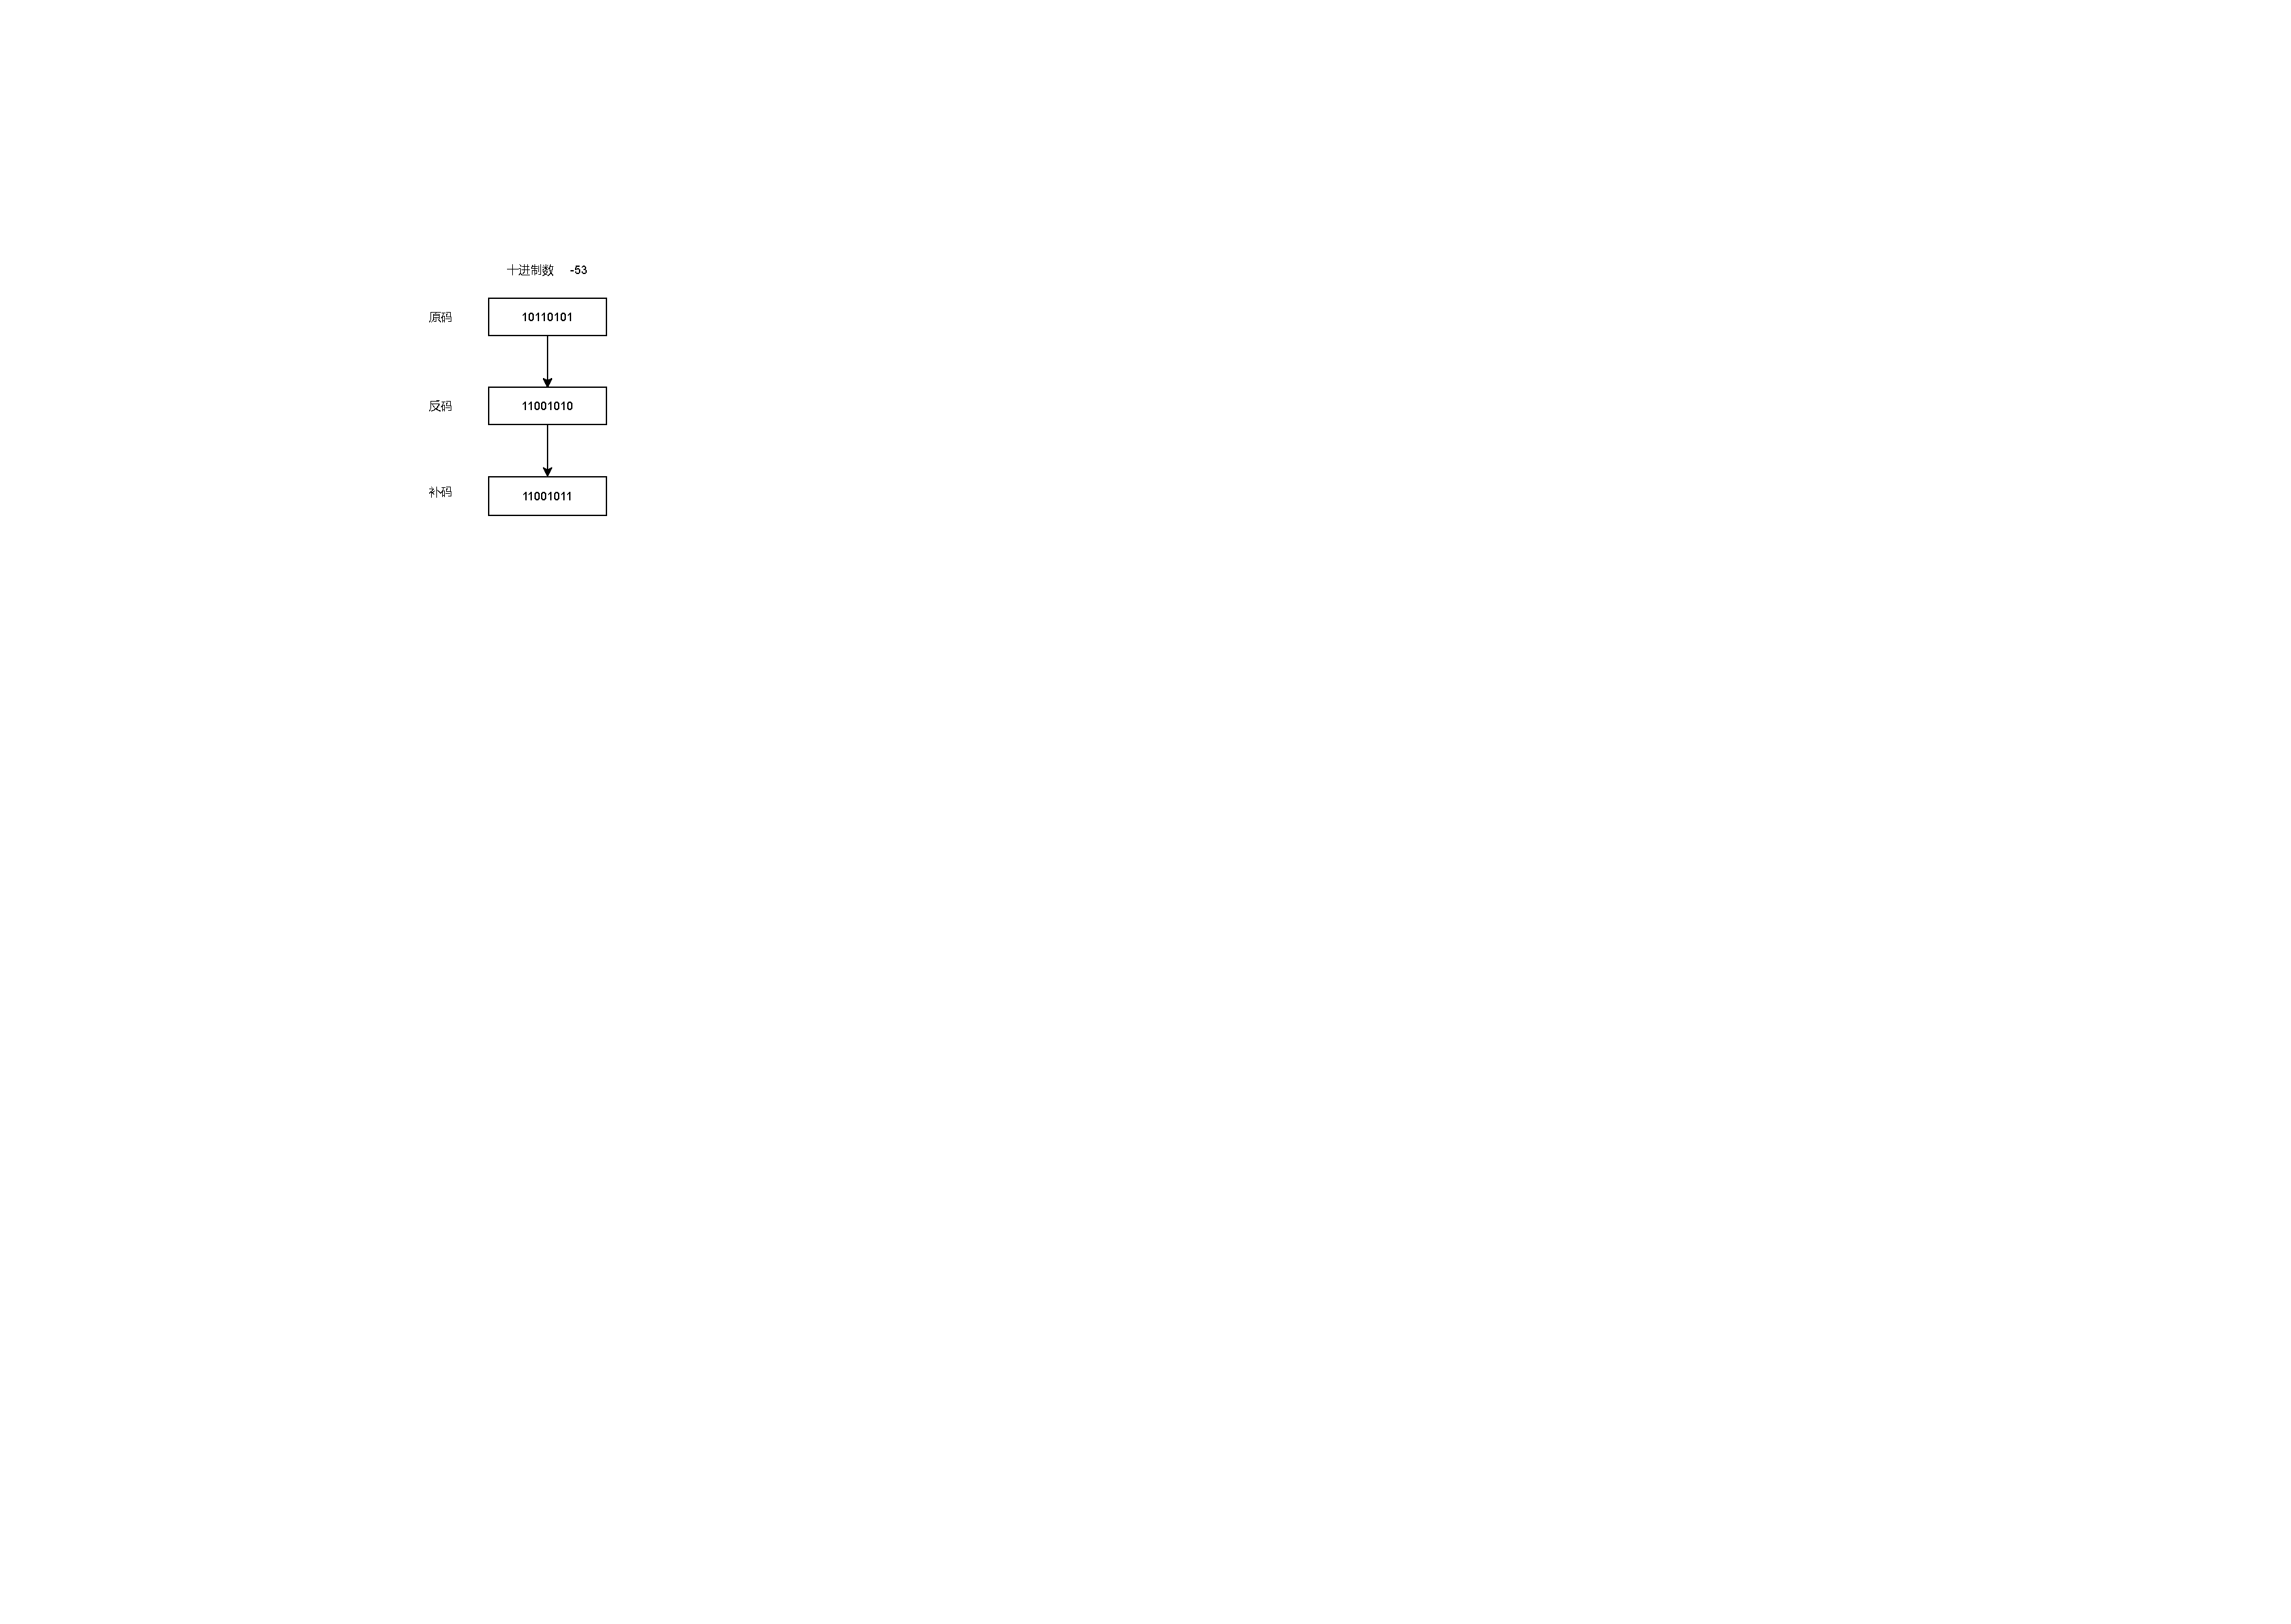
\includegraphics[width=7cm]{fig/4-fig/补码计算示意图.pdf}
  \caption{补码计算示意图}
  \label{fig:补码计算示意图}
\end{figure}

\subsection{乘除转换转换}
在硬件的世界中,四则运算所需要的资源量关系为:除法>乘法>加(减)法,导致性能下降的程度关系为:除法>乘法>加(减)法,但是其中有一个特殊情形,即2次幂乘法或除法,由于二进制数第nbit表示的十进制数大小为$2^{n-1}$,这说明距离为l的两个bit位其对应的倍数关系为$2^{l}$,所以如果是2的n次幂的乘法或除法,只需要将二进制数左移(对应乘法)或者右移(对应除法)nbit即可,移位操作在硬件中是非常容易实现的,所以这并不会使用大量的硬件资源或者降低性能。而对于非2的n次幂的乘法或除法,可以转换为多个2的幂次方乘加,然后转换为移位操作。例如$A\times 19$可以转换为$A\times 16 +A\times 2+A$,之后就可以使用移位操作替换乘法。但除了上述特殊情况,其余情况在硬件设计的时候需要尽可能避免除法的使用,并且减少乘法的使用。

由于在粒子群算法的适应度计算时采用的是均方根误差,而均方根误差的计算公式如式\eqref{eq:均方根误差计算公式}所示,是需要进行一次除N的操作的,这个N取决于粒子群算法设置的种群个体数。由前文所述,如果这个N是2的幂乘法,那么就可以将除法的操作转变为移位操作,所以本文推荐粒子群算法的种群个体数设置为16、32、64、128,这样在计算均方根误差时只需要将数据右移4、5、6、7位即可。

\subsection{四舍五入方案}
软件层面进行四舍五入非常简单,只需要判断是否小于阈值即可,放在硬件层面,判断数值是否小于阈值对应的基本逻辑单元是比较器,常见的基本逻辑单元面积关系为:加法器>比较器>选择器,比较器的面积不大不小,所以如果能减少比较器的使用数量,也能在资源消耗上带来一定收益。

所以本文进行四舍五入时采用如下方案:假设是在判断小数部分是否需要四舍五入时,即判断低8bit是否需要像第9bit进位时,可以将数值加上8'b10000000,然后右移8位即可。这么做的原理是如果需要判断低8bit是否需要四舍五入,其实只需要判断第8bit的值是否为1,如果为1,那么这个数值是一定大于8bit数最大值(255)的一半的,这时就需要进位,然后进行移位即可舍去由于加法而导致的多余数据;如果第8bit为0,那么即使加上8'b10000000也不会产生进位,进行移位后即可以完成舍入过程。而加上一个2的幂次方是可以通过异或门实现,这样做就可以减少资源消耗了。

\section{硬化前后的算法验证框架}
\subsection{进制转换与字符串操作}
由于补偿算法使用matlab编写,并且对应的硬化后的算法参考模型也是使用matlab编写的,而matlab本身对二进制计算并不友好,所以模型验证时采用了多次进制转换与字符串操作,这些操作使用matlab自带的dec2hex、hex2dec、bin2dec、num2str等函数。

\subsection{RTL model验证框架}
RTL model的验证框架示意图如图所示,三角箭头表示类型为数值,蓝色线条代表进制为十六进制,绿色线条代表进制为二进制,黑色线条代表该处为其他类型操作(比较、控制等)。验证框架主要由4部分组成:stimulator、RTL model、software、scoreboard。其中stimulator主要功能为产生测试激励,主要包含driver和monitor两个部件,monitor进行激励产生的控制,driver产生受控的测试激励。RTL model为硬化后的粒子群算法,包含三个部件:fitnesee$\_$cal(进行适应度的计算)、velocity$\_$upda(进行速度和位置的更新)、population$\_$upda(进行种群信息的更新),三者的输出都是十六进制类型的数值,输入都是二进制类型的数值,所以在上一级模块输出和下一级模块输入之间需要进行进制的转换,但在三个模块内部计算时所有数据都为十进制。software软件版本的粒子群算法,即上文中用于实验中的补偿程序,RTL model中每一部分在software中都有对应部分,作为验证RTL model正确性时的参考模型。scoreboard为得分板,比较RTL model和software的输出是否一致,并在误差大小超出设定阈值是进行报错。
\begin{figure}[htb]
  \centering
  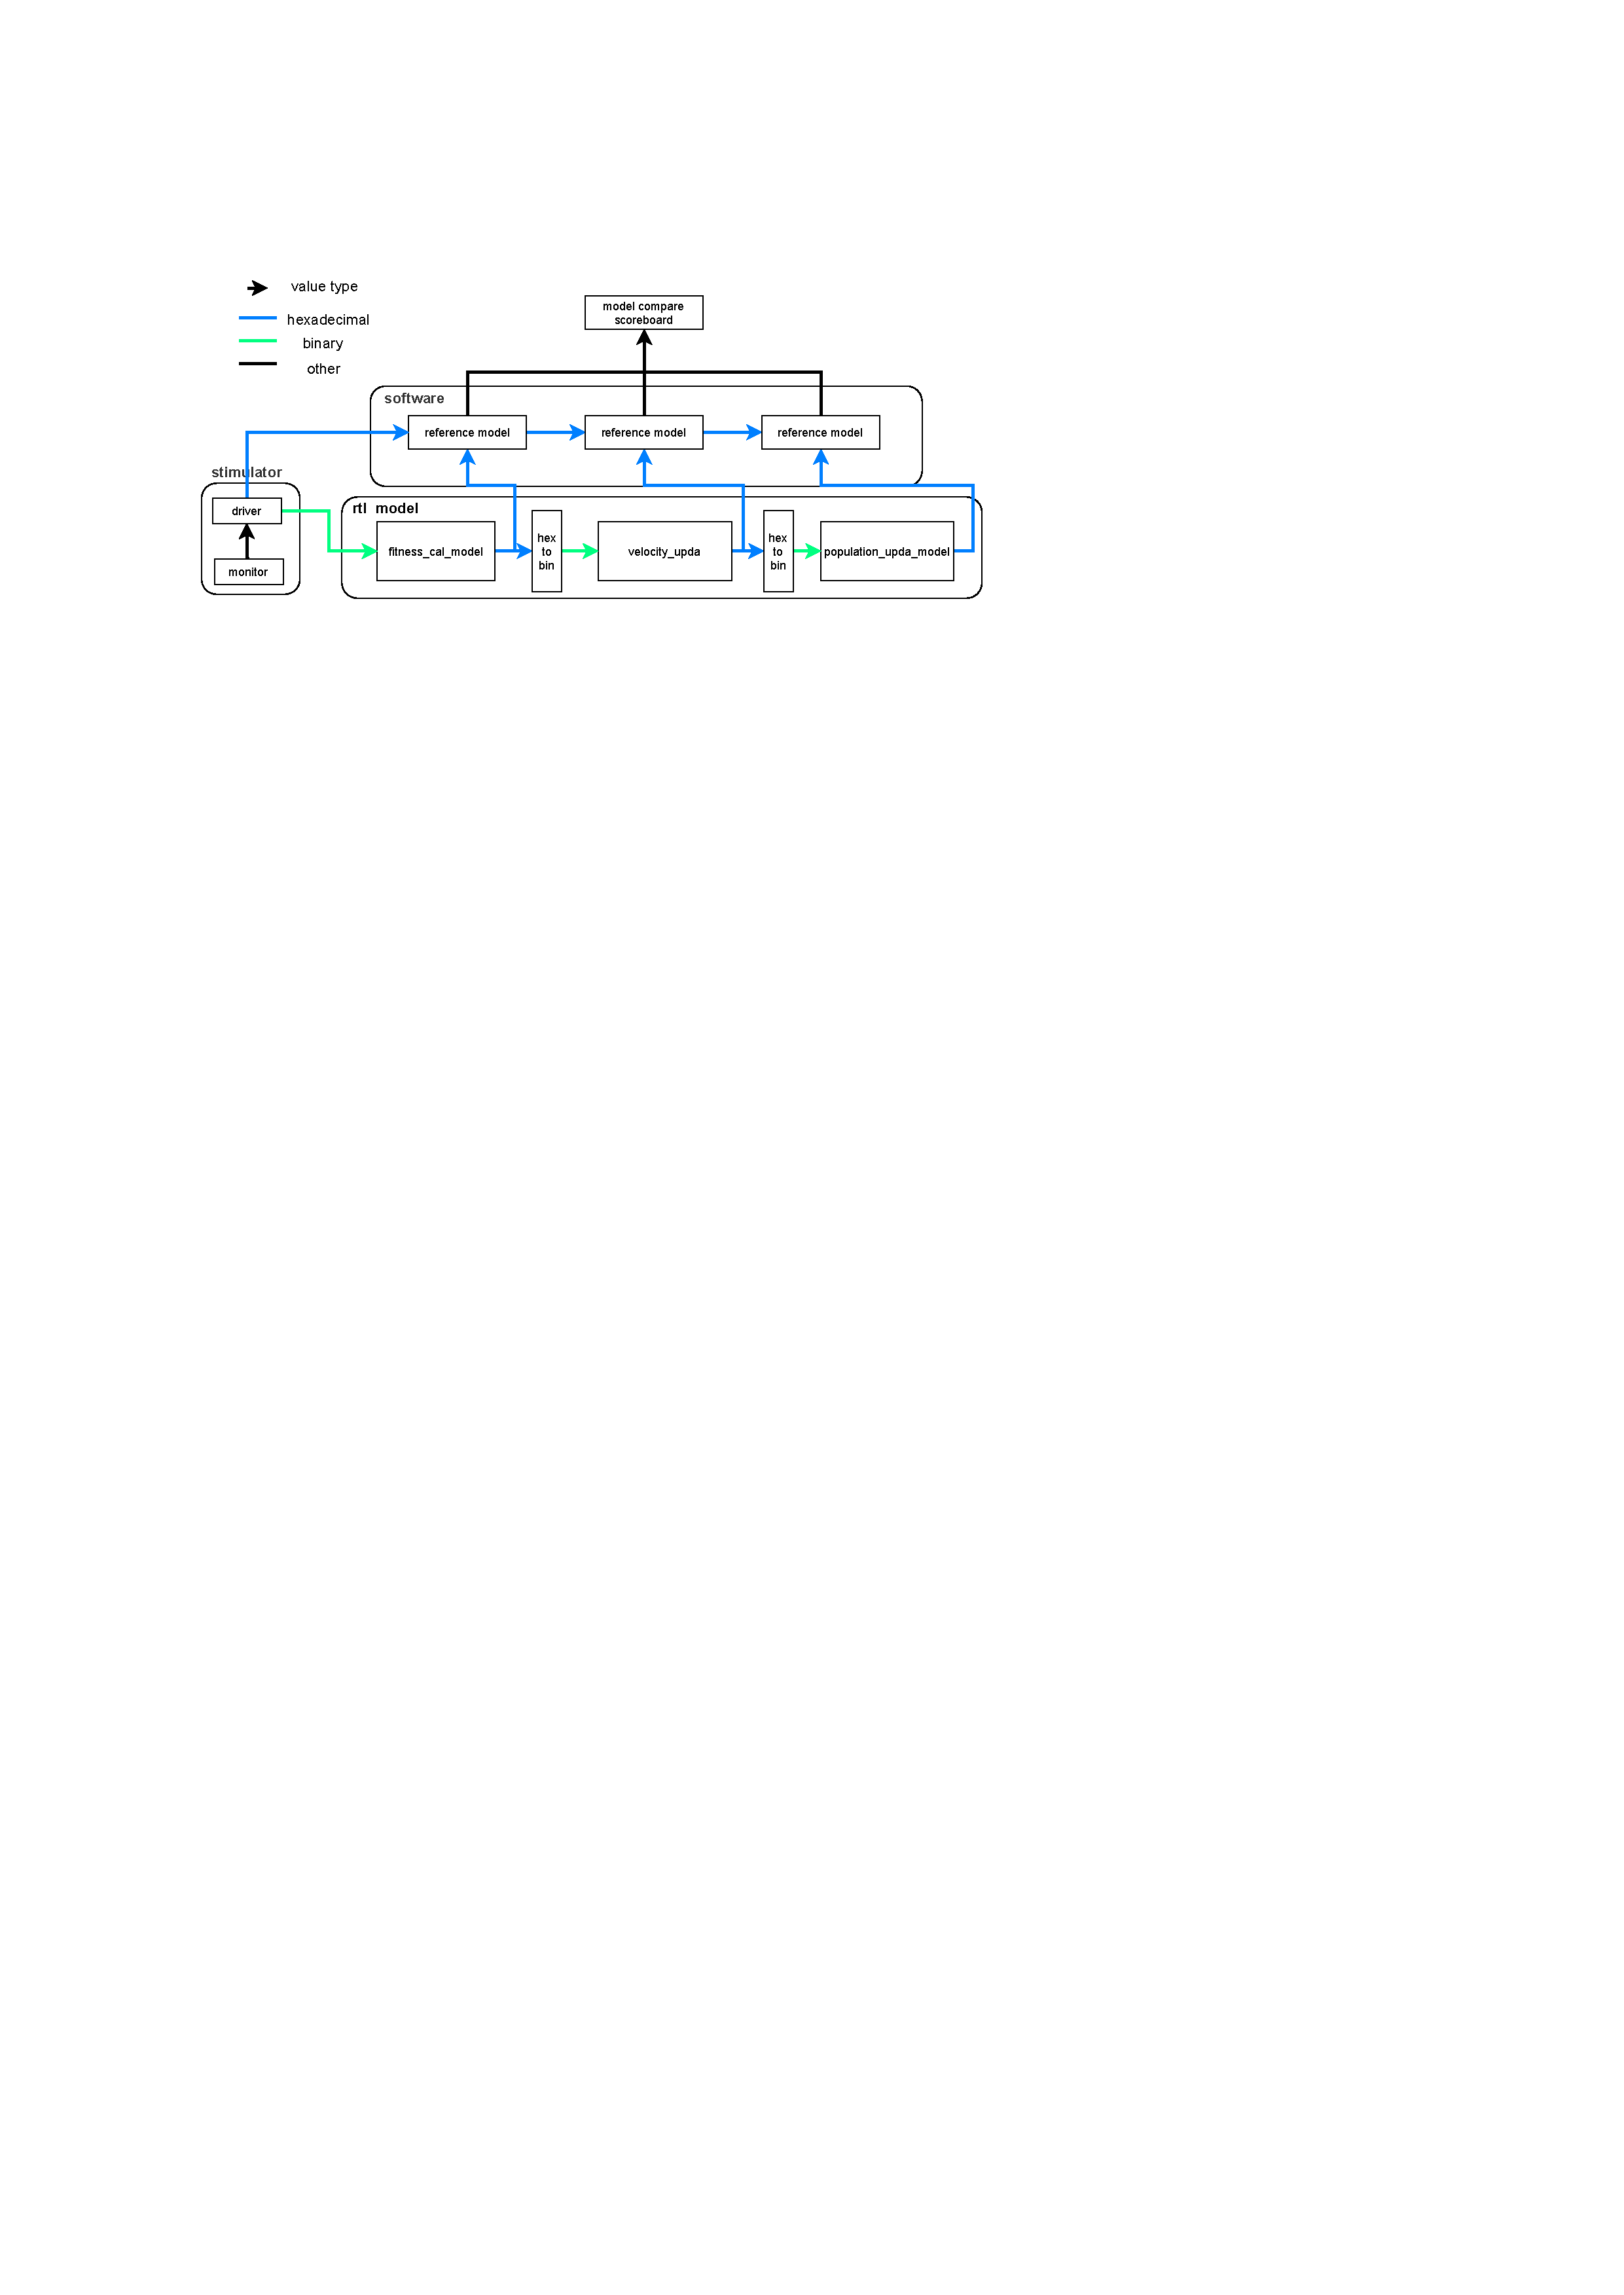
\includegraphics[width=14cm]{fig/4-fig/rtl_model验证环境.pdf}
  \caption{RTL model验证框架}
  \label{fig:RTL model验证框架}
\end{figure}

\subsection{验证激励和结果}
在单独模块的随机验证时(即每个模块的输入都是随机产生的,不来自上一模块,位移、温度、气压三个激励除外),激励产生约束如表所示。而在进行整个流水线的综合验证时,位移、气压和温度数据就采用实际的测量数据,初始搜索点则采用原始的Edlen公式,每一级模块的输入使用上一级模块的输出。
\begin{table}[H]
  \centering
  \caption{RTL model激励产生约束}
  \label{tab:RTL model激励产生约束}
  \begin{tabular}{c|c|c|c}
      \hline
      激励名                             & 激励意义                   &  数值范围       & 约束条件  \\ \hline
      fitness$\_$cal$\_$disp            & 输入的位移                  &  [-500,500]     & 无      \\ \hline
      fitness$\_$cal$\_$pres            & 输入的气压                  &  [-500,500]     & 无      \\ \hline
      fitness$\_$cal$\_$temp            & 输入的温度                  &  [-500,500]     & 无      \\ \hline
      fitness$\_$cal$\_$para            & 当前搜索点                  &  [-500,500]     & 无      \\ \hline
      population$\_$upda$\_$gbest       & 迭代结果的全局最优解         &  [0,5000]       & 无       \\ \hline
      population$\_$upda$\_$pbest       & 迭代结果的局部最优解         &  [0,5000]       &小于population$\_$upda$\_$pbest \\ \hline
      velocity$\_$upda$\_$curpara       & 上一轮迭代的位置信息         & [-500,500]      & 等于fitness$\_$cal$\_$para     \\ \hline
      velocity$\_$upda$\_$lastv         & 上一轮迭代的速度增量         & [0,1]           & 无     \\ \hline
      velocity$\_$upda$\_$randc         & 更新速度信息的随机数         & [0,1]           & 无     \\ \hline
  \end{tabular}
\end{table}

设定的最大误差阈值如下:population$\_$upda$\_$pbest模块的所有输出需要与software的输出完全一致,其余所有模块的输出的最大误差阈值为$\pm4\%$,误差产生的主要原因时上述的截断误差,截断误差虽然不大于0.0039,但截断误差一旦参与了乘法运算使得误差被放大,所以在这设定的阈值为$\pm4\%$。但需要特别强调的是,这$\pm4\%$的误差并不会给粒子群算法的结果带来太大影响,这是由于粒子群算法本身就有较大的随机性,从式\eqref{eq:粒子群算法速度更新}中两个随机数就可以看出,所以这个$\pm4\%$的误差只是又增加了一部分随机性而已,不会有太大影响。

单独模块的随机验产生了20组,每组2500个样本点,共计50000个激励测试点,而在整个流水线的综合验证时使用了所有的实际测量数据,所有验证结果的误差均为超过上述设定的阈值,可以认为算法的硬化达到了所需的要求。

\section{本章小结}
本章首先介绍了粒子群算法的基本原理以及本文使用的线性惯性权值递减策略,指出粒子群算法本身具有的早熟收敛问题,然后提出一种基于粒子群算法的优化的Edlen公式补偿方案,该方案将Edlen公式与粒子群算法相结合,不仅可以改善Edlen公式自身的温度不匹配、波长不匹配等问题,也可以解决粒子群算法自身早熟收敛的问题。并在第3章中的短时测量、长时测量和大范围温度变化测量中进行补偿,补偿效果较原始Edlen公式和整段式粒子群算法补偿方法均有不错的提升,但同时也在实验中发现当温度变化梯度过大时,线性形式的Edlen公式并不适用,为此又进行了其他实验,并且基于微积分的思想提出一种基于温度梯度的分段式粒子群算法补偿方法,实验验证该方法较原始Edlen公式和整段式粒子群算法补偿方法的效果均有提升,并且适用于较大温度变化梯度的情形。但该方法也有着一些不足之处,其中最为明显的时对粒子群算法的计算速度有较高的要求,为了解决该方法的不足,采用硬件加速的方法提升其运算速度,并介绍了算法的硬化方案,以及硬化算法正确性的验证框架,给出测试激励的产生条件和验证结果。
